\documentclass[11pt,fleqn]{article}

\usepackage[margin=1in]{geometry}
\usepackage{amsmath}
\usepackage{amssymb}
\usepackage{amsthm}
\usepackage{mathtools}
\usepackage{bm}
\usepackage{graphicx}
\usepackage{tikz}
\usepackage{url}
\usepackage{hyperref}
\usepackage{titlesec}

\usetikzlibrary{arrows.meta}

\titleformat{\section}
  {\normalfont\large\bfseries}
  {\thesection}{1em}{}

\renewcommand{\Im}{\mathrm{Im}}
\renewcommand{\Re}{\mathrm{Re}}
\newcommand{\ii}{\mathrm{i}}
\newcommand{\ee}{\mathrm{e}}
\newcommand{\dd}{\mathrm{d}}
\newcommand{\CC}{\mathbb C}
\newcommand{\RR}{\mathbb R}
\newcommand{\Ccell}{\mathcal C}
\newcommand{\Tspace}{\mathcal T}
\newcommand{\Aqp}{A_{\mathrm{QP}}}
\newcommand{\Asc}{A_{\mathrm{sc}}}
\newcommand{\Bsc}{B_{\mathrm{sc}}}
\newcommand{\Atr}{\mathcal A}
\newcommand{\Ein}{E_{\mathrm{in}}}
\newcommand{\Eout}{E_{\mathrm{out}}}
\newcommand{\Din}{D_{\mathrm{in}}}
\newcommand{\Nin}{N_{\mathrm{in}}}
\newcommand{\Dout}{D_{\mathrm{out}}}
\newcommand{\Nout}{N_{\mathrm{out}}}
\newcommand{\sigmin}{\sigma_{\min}}
\newcommand{\GammaR}{\Gamma_{\mathrm R}}
\newcommand{\FigurePlaceholder}[1]{%
  \begin{center}
    \setlength{\fboxsep}{1.2em}%
    \fbox{\parbox{0.75\textwidth}{\centering #1}}%
  \end{center}%
}
\newcommand{\SafeIncludeGraphics}[2][]{%
  \IfFileExists{#2}{%
    \includegraphics[#1]{#2}%
  }{%
    \FigurePlaceholder{Missing figure: \url{#2}}%
  }%
}
\DeclareMathOperator{\diag}{diag}
\DeclareMathOperator{\rank}{rank}

\theoremstyle{definition}
\newtheorem{definition}{Definition}
\newtheorem{conjecture}{Conjecture}
\newtheorem{theorem}{Theorem}
\newtheorem{lemma}{Lemma}

\theoremstyle{remark}
\newtheorem{remark}{Remark}

\title{A Boundary Integral Trace-Subspace Formulation for Periodic Line-Defect Waveguides}
\author{}
\date{}

\begin{document}
\maketitle

\section{Introduction}

\section{Model problem}
\label{sec:model-problem}
We consider the Helmholtz equation for a line-defect waveguide in a periodic medium: 
\begin{align}
 \Delta u(x, y) + k^2 n(x, y)^2 u(x, y) &= 0, \quad (x, y) \in \mathbb{R}^2 \setminus \text{interface}, \label{eq:helmholtz-equation}
\end{align}
and the TM mode yields the following transmission conditions on the interface \begin{align}
  u, u_\nu \text{ continuous across the interface.} \label{eq:transmission-conditions}
\end{align}
The problem geometry is a line-defect crytal (see Figure~\ref{fig:y-periodic-configuration}), we
define \begin{align*}
  \mathcal{C}^\pm_{ij} = \mathcal{C}^\pm \pm ((i-1)L^\pm, (j-1)d), \quad
  \mathcal{C}^0_j = \mathcal{C}^0 + (0, (j-1)d),\quad (i,j) \in \mathbb{Z}^2,
\end{align*}
where the unit periodicity cells are \begin{align*}
  &\mathcal{C}^\pm = \{ (x, y) | X^\pm \leq \pm x \leq X^\pm + L^\pm, 0 \leq y \leq d \},\\
  &\mathcal{C}^0 = \{ (x, y) | X^- \leq x \leq X^+, 0 \leq y \leq d \}.
\end{align*}
Let $\Omega^\pm, \Omega^0$ be the inclusions in the unit periodicity cells $\mathcal{C}^\pm, \mathcal{C}^0$, respectively, and define \begin{align*}
  \Omega^\pm_{ij} = \Omega^\pm \pm ((i-1)L^\pm, (j-1)d), \quad
  \Omega^0_j = \Omega^0 + (0, (j-1)d),\quad (i,j) \in \mathbb{Z}^2.
\end{align*}
Throughout this work, we assume that each reference inclusion is compactly
contained in the interior of its corresponding cell. More precisely, there
exists a fixed constant \(\delta_\Omega>0\) such that
\begin{align*}
  \overline{\Omega^s}&\subset\operatorname{int}(\mathcal C^s),
  &\operatorname{dist}\!\left(\overline{\Omega^s},\partial\mathcal C^s\right)
  &\geq\delta_\Omega,
  &&s\in\{-,0,+\}.
\end{align*}
Consequently, every translated inclusion remains a positive distance from the
boundary of its translated cell, and distinct periodic copies do not touch.
Then the interface in \eqref{eq:transmission-conditions} is \begin{align*}
  \bigcup_{(i,j) \in \mathbb{Z}^2} \partial\Omega^\pm_{ij} \cup
  \bigcup_{j \in \mathbb{Z}} \partial\Omega^0_j.
\end{align*}
The refractive index $n(x, y)$ is a piecewise constant function defined as \begin{align}
  n(x,y) = \begin{cases}
    n^+, & (x,y) \in \Omega^+_{ij},\\
    n^-, & (x,y) \in \Omega^-_{ij},\\
    n^0, & (x,y) \in \Omega^0_j,\\
    1, & \text{otherwise},
  \end{cases}
\end{align}

\begin{figure}[ht]
\centering
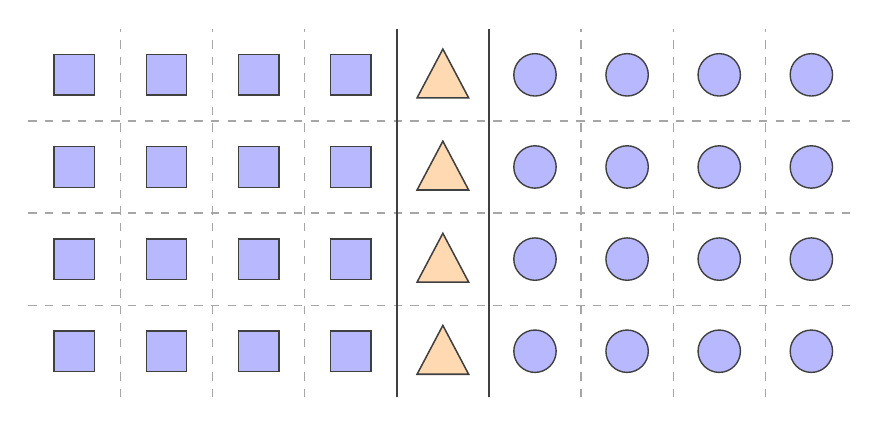
\begin{tikzpicture}[
  x=1.17cm,
  y=1.17cm,
  gridline/.style={draw=black!35, dashed, line width=0.45pt},
  defectline/.style={draw=black!75, line width=0.8pt},
  leftinclusion/.style={draw=black!75, fill=blue!28, line width=0.5pt},
  centerinclusion/.style={draw=black!75, fill=orange!30, line width=0.55pt},
  rightinclusion/.style={draw=black!75, fill=blue!28, line width=0.5pt}
]
  \foreach \x in {-3.5,-2.5,-1.5,1.5,2.5,3.5} {
    \draw[gridline] (\x,-2) -- (\x,2);
  }
  \foreach \y in {-1,0,1} {
    \draw[gridline] (-4.5,\y) -- (4.5,\y);
  }
  \draw[defectline] (-0.5,-2) -- (-0.5,2);
  \draw[defectline] (0.5,-2) -- (0.5,2);

  \foreach \x in {-4,-3,-2,-1} {
    \foreach \y in {-1.5,-0.5,0.5,1.5} {
      \draw[leftinclusion] (\x-0.22,\y-0.22) rectangle ++(0.44,0.44);
    }
  }
  \foreach \x in {1,2,3,4} {
    \foreach \y in {-1.5,-0.5,0.5,1.5} {
      \draw[rightinclusion] (\x,\y) circle [radius=0.23];
    }
  }
  \foreach \y in {-1.5,-0.5,0.5,1.5} {
    \draw[centerinclusion] (-0.28,\y-0.25) -- (0.28,\y-0.25) -- (0,\y+0.28) -- cycle;
  }
\end{tikzpicture}
\caption{Example of configuration.}
\label{fig:y-periodic-configuration}
\end{figure}

Now we state the eigenvalue problem, an eigensolution is defined as 
\begin{definition}
An eigensolution is non-trivial solution to \eqref{eq:helmholtz-equation} and \eqref{eq:transmission-conditions} with the following conditions:
\begin{align*}
  &u(x, y + d) = e^{\ii\beta d}u(x, y),\quad \forall (x,y) \in \mathbb{R}^2\\
  &u(x,y)\to 0 \quad \text{as } x\to\pm\infty, \text{ for } y\in[0,d],
\end{align*}
where $\beta$ is the \emph{Bloch wavenumber}.
\end{definition}

For a prescribed Bloch wavenumber $\beta$, the eigenvalue problem is to
determine a spectral parameter $k$ for which there exists a nonzero field
$u$ that is an eigensolution in the sense of Definition~1. Equivalently,
we seek $k$ and $u\not\equiv 0$ satisfying
$(k,u)$ with $u \not\equiv 0$ such that
\begin{align}
  \begin{cases}
  &\Delta u + k^2 n^2 u = 0
    \quad \text{in } \mathbb{R}^2 \setminus
    \left(
      \bigcup_{(i,j) \in \mathbb{Z}^2} \partial\Omega^\pm_{ij}
      \cup
      \bigcup_{j \in \mathbb{Z}} \partial\Omega^0_j
    \right),\\
  &u \text{ and } u_\nu \text{ are continuous across each interface},\\
  &u(x,y+d)=e^{\ii\beta d}u(x,y),\\
  &u(x,y)\to 0 \quad \text{as } x\to\pm\infty,
    \text{ for } y\in[0,d].
  \end{cases}
  \label{eq:original-eigenvalue-problem}
\end{align}
If such a nonzero field $u$ exists, the parameter pair $(k,\beta)$ is
called a \emph{Bloch eigenvalue} of the line-defect waveguide, and $u$ is called
an associated eigensolution.

\section{Reduction to a bounded domain}


\begin{figure}[ht]
\centering
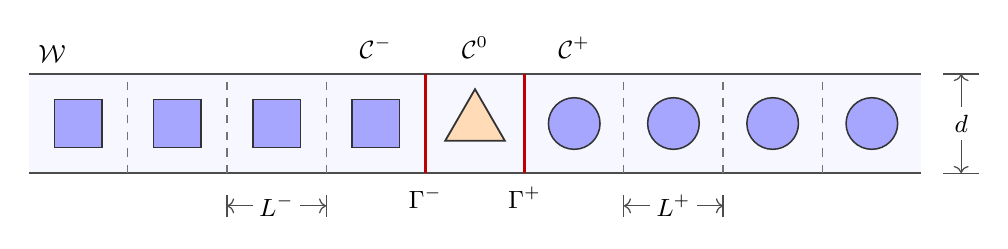
\begin{tikzpicture}[
  x=1.26cm,
  y=1.26cm,
  every node/.style={font=\small},
  stripfill/.style={fill=blue!3},
  stripedge/.style={draw=black!70, line width=0.65pt},
  interface/.style={draw=black!55, dashed, line width=0.45pt},
  obstacle/.style={draw=black!80, fill=blue!35, line width=0.55pt},
  defect/.style={draw=black!80, fill=orange!28, line width=0.65pt},
  port/.style={draw=red!75!black, line width=1.0pt},
  dimtick/.style={draw=black!70, line width=0.45pt},
  dimarrow/.style={->, draw=black!70, line width=0.45pt}
]
  \fill[stripfill] (-4.5,-0.5) rectangle (4.5,0.5);
  \draw[stripedge] (-4.5,-0.5) -- (4.5,-0.5);
  \draw[stripedge] (-4.5,0.5) -- (4.5,0.5);
  \foreach \x in {-3.5,-2.5,-1.5,1.5,2.5,3.5} {
    \draw[interface] (\x,-0.5) -- (\x,0.5);
  }

  \foreach \x in {-4,-3,-2,-1} {
    \draw[obstacle] (\x-0.24,-0.24) rectangle ++(0.48,0.48);
  }
  \draw[defect] (-0.30,-0.173) -- (0.30,-0.173) -- (0,0.346) -- cycle;
  \foreach \x in {1,2,3,4} {
    \draw[obstacle] (\x,0) circle [radius=0.26];
  }

  \draw[port] (-0.5,-0.5) -- (-0.5,0.5);
  \draw[port] (0.5,-0.5) -- (0.5,0.5);
  \node[below] at (-0.5,-0.54) {$\Gamma^-$};
  \node[below] at (0.5,-0.54) {$\Gamma^+$};
  \node[above right] at (-4.5,0.52) {$\mathcal W$};
  \node[above] at (-1,0.56) {$\mathcal C^-$};
  \node[above] at (0,0.56) {$\mathcal C^0$};
  \node[above] at (1,0.56) {$\mathcal C^+$};

  \draw[dimtick] (4.72,-0.5) -- (5.08,-0.5);
  \draw[dimtick] (4.72,0.5) -- (5.08,0.5);
  \draw[dimarrow] (4.9,0.17) -- (4.9,0.5);
  \draw[dimarrow] (4.9,-0.17) -- (4.9,-0.5);
  \node[fill=white, inner sep=1.2pt] at (4.9,0) {$d$};

  \draw[dimtick] (-2.5,-0.72) -- (-2.5,-0.94);
  \draw[dimtick] (-1.5,-0.72) -- (-1.5,-0.94);
  \draw[dimarrow] (-2.24,-0.83) -- (-2.5,-0.83);
  \draw[dimarrow] (-1.76,-0.83) -- (-1.5,-0.83);
  \node[fill=white, inner sep=1.6pt] at (-2,-0.83) {$L^-$};

  \draw[dimtick] (1.5,-0.72) -- (1.5,-0.94);
  \draw[dimtick] (2.5,-0.72) -- (2.5,-0.94);
  \draw[dimarrow] (1.76,-0.83) -- (1.5,-0.83);
  \draw[dimarrow] (2.24,-0.83) -- (2.5,-0.83);
  \node[fill=white, inner sep=1.6pt] at (2,-0.83) {$L^+$};
\end{tikzpicture}
\caption{The waveguide strip.}
\label{fig:waveguide-strip}
\end{figure}

Since the Bloch wavenumber $\beta$ is prescribed, the eigenvalue problem is reduced to the 
waveguide strip $\mathcal{W} = \mathbb{R} \times [0, d]$ in Figure~\ref{fig:waveguide-strip}, and we will use the new notation: \begin{align*}
  &\mathcal{C}^\pm_j = \mathcal{C}^\pm \pm ((j-1)L^\pm, 0),\\
  &\Omega^\pm_j = \Omega^\pm \pm ((j-1)L^\pm, 0),\quad \Sigma^\pm = \bigcup_{j\in\mathbb{Z}} \partial\Omega^\pm_j,\quad \Sigma = \Sigma^+ \cup \Sigma^- \cup \partial \Omega^0\\
  &\Gamma^\pm = \{x = X^\pm\} \times [0,d],\quad \Gamma^\pm_j = \{x = X^\pm \pm (j-1)L^\pm\} \times [0,d].
\end{align*}
The we can rewrite the eigenvalue problem as follows:
\begin{align}
\begin{cases}
  &\Delta u + k^2 n^2 u = 0 \quad \text{in } \mathcal{W}\setminus \Sigma,\\
  &u|_{y = d} = e^{\ii\beta d} u|_{y = 0}, \quad \partial_y u|_{y = d} = e^{\ii\beta d} \partial_y u|_{y = 0},\\
  &u(x,y)\to 0 \quad \text{as } x\to\pm\infty,
    \text{ for } y\in[0,d],\\
  &u, u_\nu \text{ continuous across } \Sigma.
\end{cases}
\end{align}

Our goal is to reduce the problem to the bounded domain $\mathcal C^0$
by imposing exact nonlocal boundary conditions on the artificial
boundaries $\Gamma^\pm$. Formally, these boundary conditions may be
written in terms of Dirichlet-to-Neumann operators $\Lambda^\pm$ as
\begin{align}
\begin{cases}
  &\Delta u + k^2 n^2 u = 0 \quad \text{in } \mathcal{C}^0\setminus \partial \Omega^0,\\
  &u|_{y = d} = e^{\ii\beta d} u|_{y = 0}, \quad \partial_y u|_{y = d} = e^{\ii\beta d} \partial_y u|_{y = 0},\\
  &\partial_x u |_{\Gamma^\pm} \mp \Lambda^\pm u|_{\Gamma^\pm} = 0,\\
  &u, u_\nu \text{ continuous across } \partial \Omega^0.
\end{cases}\label{eq:dtn-cell-problem}
\end{align}
The precise definition of $\Lambda^\pm$, the assumptions under which
these operators are well-defined, and their equivalent interpretation
in terms of outgoing Cauchy trace subspaces will be given in
Section~\ref{sec:outgoing-trace-subspaces}. In the subsequent formulation, we will not construct the DtN operators
explicitly. Instead, we impose the equivalent outgoing trace-subspace
condition directly.

\subsection{Outgoing trace subspaces}\label{sec:outgoing-trace-subspaces}
In this subsection we show how to interpret the radiation condition in terms of outgoing trace subspaces. 
\begin{definition}
  For a sufficiently regular field \(u\), its Cauchy \emph{trace} on the artificial boundaries $\Gamma^\pm_j$ is
  \[
    \operatorname{Tr}_{\Gamma^\pm_j}u
    =
    \begin{bmatrix}
      u|_{\Gamma^\pm_j}\\
      \pm \partial_x u|_{\Gamma^\pm_j}
    \end{bmatrix}
    \in
    H^{1/2}_\beta(\Gamma^\pm_j)\times H^{-1/2}_\beta(\Gamma^\pm_j),
  \]
  where the subscript \(\beta\) indicates the \(y\)-quasiperiodic trace space.
\end{definition}

Let $\mathcal{W}^+ = [X^+, +\infty) \times [0,d]$ and $\mathcal{W}^- = (-\infty, X^-] \times [0,d]$ be the semi-infinite periodic half-guides. For fixed $(k, \beta)$, define $\mathcal{U}^\pm(k,\beta)$ as the space of fields $u^\pm$ satisfying the following equations:
\begin{align*}
\begin{cases}
  &\Delta u^\pm + k^2 n^2 u^\pm = 0 \quad \text{in } \mathcal{W^\pm}\setminus \Sigma^\pm,\\
  &u^\pm|_{y = d} = e^{\ii\beta d} u^\pm|_{y = 0}, \quad \partial_y u^\pm|_{y = d} = e^{\ii\beta d} \partial_y u^\pm|_{y = 0},\\
  &u^\pm(x,y)\to 0 \quad \text{as } x\to \pm\infty,
    \text{ for } y\in[0,d],\\
  &u^\pm, u^\pm_\nu \text{ continuous across } \Sigma^\pm.
\end{cases}
\end{align*}
Then the \emph{outgoing trace subspace} on $\Gamma^\pm$ is defined by\begin{align}
  \mathcal{E}^\pm_{\rm out}(k,\beta) :=
  \left\{
    \operatorname{Tr}_{\Gamma^\pm}u^\pm :
    u^\pm\in \mathcal{U}^\pm(k,\beta)
  \right\}
  \subset H^{1/2}_\beta(\Gamma^\pm)\times H^{-1/2}_\beta(\Gamma^\pm).
\end{align}

We now relate this definition to the usual Dirichlet-to-Neumann map. Let
\[
  \pi_\mathrm{D}
  \begin{bmatrix}
    D\\ N
  \end{bmatrix}
  =D,
  \qquad
  \pi_\mathrm{N}
  \begin{bmatrix}
    D\\ N
  \end{bmatrix}
  =N
\]
be the Dirichlet and Neumann projections from the Cauchy trace space. If, for the
half-guide problem, every admissible Dirichlet trace \(D^\pm\in H^{1/2}_\beta(\Gamma^\pm)\)
has a unique outgoing extension \(u^\pm\in\mathcal U^\pm(k,\beta)\), then the DtN map is
defined by
\[
  \Lambda^\pm(k,\beta)D^\pm
  :=
  \pi_\mathrm{N} \operatorname{Tr}_{\Gamma^\pm}u^\pm
  =
  \pm \partial_x u^\pm|_{\Gamma^\pm},
  \qquad
  u^\pm|_{\Gamma^\pm}=D^\pm .
\]
Equivalently,
\[
  \Lambda^\pm(k,\beta)
  =
  \pi_\mathrm{N}\circ
  \left(
    \pi_\mathrm{D}|_{\mathcal E^\pm_{\rm out}(k,\beta)}
  \right)^{-1}.
\]
Hence, whenever the above inverse is well-defined, the outgoing trace subspace is the
graph of the DtN map:
\[
  \mathcal E^\pm_{\rm out}(k,\beta)
  =
  \left\{
    \begin{bmatrix}
      D^\pm\\
      \Lambda^\pm(k,\beta)D^\pm
    \end{bmatrix}
    :
    D^\pm\in H^{1/2}_\beta(\Gamma^\pm)
  \right\}.
\]
Therefore the DtN boundary condition in \eqref{eq:dtn-cell-problem}
\[
  \pm \partial_x u |_{\Gamma^\pm} = \Lambda^\pm(k,\beta) u |_{\Gamma^\pm}
\]
is equivalent to the trace-subspace condition
\[
  \operatorname{Tr}_{\Gamma^\pm}u\in \mathcal E^\pm_{\rm out}(k,\beta).
\]
In this work we use the latter formulation. It keeps the Dirichlet and Neumann traces
on equal footing and avoids explicitly constructing the DtN operators. 

\begin{remark}[Absorbing DtN maps]
In the previous statement, we assume that for any $D^\pm \in H^{1/2}_\beta(\Gamma^\pm)$, there exists a unique outgoing solution $u^\pm \in \mathcal U^\pm(k,\beta)$, thus $\pi_\mathrm{D}|_{\mathcal E^\pm_{\rm out}(k,\beta)}$ is invertible. This may not be true for all $(k,\beta)$, so we consider the following absorbing case.

For $\varepsilon>0$ and prescribed
$D^\pm\in H^{1/2}_\beta(\Gamma^\pm)$, consider
\[
\begin{cases}
\Delta u_\varepsilon^\pm
+n^2(k^2+\ii\varepsilon)u_\varepsilon^\pm=0
& \text{in }W^\pm\setminus\Sigma^\pm,\\
u_\varepsilon^\pm|_{y=d}
=e^{\ii\beta d}u_\varepsilon^\pm|_{y=0},
\qquad
\partial_yu_\varepsilon^\pm|_{y=d}
=e^{\ii\beta d}\partial_yu_\varepsilon^\pm|_{y=0},\\
u_\varepsilon^\pm,\ (u_\varepsilon^\pm)_\nu
\text{ are continuous across }\Sigma^\pm,\\
u_\varepsilon^\pm|_{\Gamma^\pm}=D^\pm .
\end{cases}
\]
This absorbing half-guide problem admits a unique solution in
$H^1_\beta(W^\pm)$; see
\cite{JolyLiFliss2006,Coatleven2012}. The absorption selects a solution
that decays along the half-guide, so no additional radiation condition
is required.
Consequently, if $\mathcal E^\pm_\varepsilon(k,\beta)$ denotes its
Cauchy trace space, then
\[
\pi^\pm_{\mathrm{D},\varepsilon}
:=
\left.\pi_\mathrm{D}\right|_{\mathcal E^\pm_\varepsilon(k,\beta)}
\]
is invertible, and one may define
\[
\Lambda^\pm_\varepsilon(k,\beta)
=
\pi_\mathrm{N}\circ
\left(\pi^\pm_{\mathrm{D},\varepsilon}\right)^{-1}.
\]
The behavior of $\Lambda^\pm_\varepsilon$ as
$\varepsilon\to0^+$ is not addressed here. We therefore use the
outgoing trace-subspace formulation directly for the lossless problem.
\end{remark}

Now we rewrite
the eigenvalue problem \eqref{eq:dtn-cell-problem} in the trace-subspace formulation:
\begin{align}
\begin{cases}
  &\Delta u + k^2 n^2 u = 0 \quad \text{in } \mathcal{C}^0\setminus \partial \Omega^0,\\
  &u|_{y = d} = e^{\ii\beta d} u|_{y = 0}, \quad \partial_y u|_{y = d} = e^{\ii\beta d} \partial_y u|_{y = 0},\\
  &\operatorname{Tr}_{\Gamma^\pm} u \in \mathcal{E}^\pm_{\mathrm{out}}(k,\beta),\\
  &u, u_\nu \text{ continuous across } \partial \Omega^0.
\end{cases}
\label{eq:trace-subspace-cell-tep}
\end{align}

\begin{theorem}
  A parameter pair $(k,\beta)$ is a Bloch eigenvalue of
  \eqref{eq:original-eigenvalue-problem} if and only if the bounded
  trace-subspace problem \eqref{eq:trace-subspace-cell-tep} admits a
  nontrivial solution.
\end{theorem}

\begin{proof}
We prove the equivalence for sufficiently regular fields for which the Cauchy
traces on \(\Gamma^\pm\) are well-defined and the usual elliptic gluing
argument across these artificial interfaces is valid.

First suppose that \((k,\beta)\) is a Bloch eigenvalue of
\eqref{eq:original-eigenvalue-problem}, with eigensolution \(u\). Let
\[
  u^0:=u|_{\mathcal C^0},\qquad
  u^\pm:=u|_{\mathcal W^\pm}.
\]
The restriction \(u^0\) satisfies the Helmholtz equation, the
\(y\)-quasiperiodic boundary condition, and the transmission conditions on
\(\partial\Omega^0\). Moreover, since the full eigensolution decays as
\(x\to\pm\infty\), each \(u^\pm\) belongs to
\(\mathcal U^\pm(k,\beta)\). By the definition of the outgoing trace subspaces,
\[
  \operatorname{Tr}_{\Gamma^\pm}u^0
  =
  \operatorname{Tr}_{\Gamma^\pm}u^\pm
  \in
  \mathcal E^\pm_{\rm out}(k,\beta).
\]
Thus \(u^0\) solves \eqref{eq:trace-subspace-cell-tep}. If $u^0\equiv0$, then $u = 0$ on $\Gamma^\pm$, which implies that $u = 0$ on $\mathcal{W}^\pm$; see Theorem~3.3.1 in \cite{Isakov2017}. This
contradicts the nontriviality of the eigensolution.

Conversely, assume that \eqref{eq:trace-subspace-cell-tep} has a nontrivial
solution \(u^0\) in \(\mathcal C^0\). The trace condition means that, for each
sign, there exists \(u^\pm\in\mathcal U^\pm(k,\beta)\) such that
\[
  \operatorname{Tr}_{\Gamma^\pm}u^\pm
  =
  \operatorname{Tr}_{\Gamma^\pm}u^0.
\]
Define a field on the whole strip by
\[
  u(x,y)=
  \begin{cases}
    u^-(x,y), & (x,y)\in \mathcal W^-,\\
    u^0(x,y), & (x,y)\in \mathcal C^0,\\
    u^+(x,y), & (x,y)\in \mathcal W^+.
  \end{cases}
\]
The equality of Cauchy traces gives continuity of both the Dirichlet trace and
the outward normal derivative across \(\Gamma^\pm\). Therefore no additional
interface source is created at the artificial boundaries, and the glued field
satisfies the Helmholtz equation and the physical transmission conditions in
the whole strip. The three pieces are \(y\)-quasiperiodic with the same Bloch
phase, while the half-guide pieces decay as \(x\to\pm\infty\) by the definition
of \(\mathcal U^\pm(k,\beta)\). Hence the glued field is an eigensolution of
\eqref{eq:original-eigenvalue-problem}. It is nonzero because
\(u^0\not\equiv0\), so \((k,\beta)\) is a Bloch eigenvalue.
\end{proof}

\subsection{Rayleigh expansions in homogeneous background}
Before introducing the representation of the solutions, we recall the form of 
$y$-quasiperiodic solutions in a homogeneous background. Consider the following Helmholtz equation in an empty cell $\mathcal{C} = [X_\mathrm{L},X_\mathrm{R}] \times [0,d]$:\begin{align*}
\begin{cases}
  &\Delta u + k^2 u = 0, \quad (x, y) \in \mathcal{C},\\
  &u|_{y = d} = e^{\ii\beta d} u|_{y = 0}, \quad \partial_y u|_{y = d} = e^{\ii\beta d} \partial_y u|_{y = 0}.
\end{cases}
\end{align*}
Define \begin{align*}
  \beta_m = \beta + \frac{2\pi m}{d},\quad \psi_m(y) = \frac{1}{\sqrt{d}} e^{\ii \beta_m y},\quad m \in \mathbb{Z},
\end{align*}
then a $y$-quasiperiodic field with period $d$ can be expanded in the $\beta$-quasiperiodic Fourier basis $\{\psi_m\}_{m \in \mathbb{Z}}$ as 
\begin{align*}
  u(x,y) = \sum_{m\in\mathbb{Z}} u_m(x) \psi_m(y).
\end{align*}
Substituting this expansion into the homogeneous Helmholtz equation yields 
\begin{align}
  u(x,y)= \sum_{m\in\mathbb Z} \xi_m^\rightarrow e^{\ii\gamma_m x}\psi_m(y) + 
  \sum_{m\in\mathbb Z} \xi_m^\leftarrow e^{-\ii\gamma_m x}\psi_m(y),
  \label{eq:rayleigh-expansion}
\end{align}
where $\gamma_m$ is chosen as follows: \begin{align*}
  \gamma_m = \begin{cases}
    \sqrt{k^2 - \beta_m^2}, & k^2 \geq \beta_m^2,\\
    \ii\sqrt{\beta_m^2 - k^2}, & k^2 < \beta_m^2.
  \end{cases}
\end{align*}
The expansion \eqref{eq:rayleigh-expansion} is called the \emph{Rayleigh expansion}, and the coefficients $\xi = (\xi^\leftarrow, \xi^\rightarrow)$ are called the Rayleigh coefficients \cite{Arens2006}; in some literature, expansion \eqref{eq:rayleigh-expansion} is also called the Rayleigh-Bloch expansion \cite{Wilcox1984}, we use the former terminology in this work. And we call the corresponding field 
$u$ a Rayleigh field.

\begin{definition}[Wood anomaly]
A parameter pair $(k,\beta)$ is said to be at a \emph{Wood anomaly}
if
\[
  \gamma_m(k,\beta)=0
\]
for some $m\in\mathbb Z$, or equivalently,
\[
  k=\left|\beta+\frac{2\pi m}{d}\right|
\]
for some $m\in\mathbb Z$.
\end{definition}

Assume that \((k,\beta)\) is not at a Wood anomaly. If
\(u\in H^1_\beta(\mathcal C)\) is a weak solution of the homogeneous
Helmholtz equation, then there exist unique Rayleigh coefficient
sequences \(\xi^\rightarrow\) and \(\xi^\leftarrow\) such that the following
series converges to \(u\) in \(H^1(\mathcal C)\):
\begin{align}
u(x,y)=
\sum_{m\in\mathbb Z}
\left(
\xi_m^\rightarrow e^{\ii\gamma_m (x - X_*)}
+
\xi_m^\leftarrow e^{-\ii\gamma_m (x - X_*)}
\right)\psi_m(y),
\label{eq:rayleigh-expansion-centered}
\end{align}
At the reference cross-section \(x=X_*\), orthonormality of
\(\{\psi_m\}_{m\in\mathbb Z}\) gives
\begin{align*}
  \int_0^d u(X_*,y)\overline{\psi_m(y)}\,\dd y
  &=\xi_m^\rightarrow+\xi_m^\leftarrow,\\
  \int_0^d \partial_xu(X_*,y)\overline{\psi_m(y)}\,\dd y
  &=\ii\gamma_m\bigl(\xi_m^\rightarrow-\xi_m^\leftarrow\bigr).
\end{align*}
Since \(\gamma_m\neq0\), solving these two equations yields the explicit
coefficient formulas
\begin{align}
  \xi_m^\rightarrow = \xi_m^\rightarrow(X_*)
  &=\frac{1}{2}\int_0^d
  \left(
    u(X_*,y)+\frac{1}{\ii\gamma_m}\partial_xu(X_*,y)
  \right)\overline{\psi_m(y)}\,\dd y,
  \label{eq:right-coefficient-extraction}
  \\
  \xi_m^\leftarrow = \xi_m^\leftarrow(X_*)
  &=\frac{1}{2}\int_0^d
  \left(
    u(X_*,y)-\frac{1}{\ii\gamma_m}\partial_xu(X_*,y)
  \right)\overline{\psi_m(y)}\,\dd y,
  \qquad m\in\mathbb Z.
  \label{eq:left-coefficient-extraction}
\end{align}
Although the numerical values of the Rayleigh coefficients depend on the
chosen reference cross-section, their vanishing does not. More precisely, if
the reference is changed from \(X_*\) to \(X_*'\), then
\[
  \xi_m^\rightarrow(X_*')
  =e^{\ii\gamma_m(X_*'-X_*)}\xi_m^\rightarrow(X_*),
  \qquad
  \xi_m^\leftarrow(X_*')
  =e^{-\ii\gamma_m(X_*'-X_*)}\xi_m^\leftarrow(X_*).
\]
\begin{definition}[Rayleigh radiation condition]
\label{def:rayleigh-radiation-condition}
Let \(\mathcal C=[X_\mathrm{L},X_\mathrm{R}]\times[0,d]\) be a cell
containing an inclusion \(\Omega\), and assume that \((k,\beta)\) is not at a
Wood anomaly. Let \(u\) be a sufficiently regular \(y\)-quasiperiodic field
satisfying
\[
  (\Delta+k^2)u=0
  \qquad\text{in }\mathcal C\setminus\overline\Omega.
\]
We say that \(u\) satisfies the \emph{Rayleigh radiation condition} if its
incoming Rayleigh coefficients vanish at both vertical boundaries, namely,
\[
  \xi_m^\rightarrow(u;X_\mathrm{L})=0,
  \qquad
  \xi_m^\leftarrow(u;X_\mathrm{R})=0,
  \qquad m\in\mathbb Z.
\]
Equivalently, the Cauchy data of \(u\) satisfy
\begin{align}
  \int_0^d
  \left(
    u(X_\mathrm{L},y)
    +\frac{1}{\ii\gamma_m}\partial_xu(X_\mathrm{L},y)
  \right)\overline{\psi_m(y)}\,\dd y
  &=0,
  \qquad m\in\mathbb Z,
  \label{eq:left-outgoing-rayleigh-condition}\\
  \int_0^d
  \left(
    u(X_\mathrm{R},y)
    -\frac{1}{\ii\gamma_m}\partial_xu(X_\mathrm{R},y)
  \right)\overline{\psi_m(y)}\,\dd y
  &=0,
  \qquad m\in\mathbb Z,
  \label{eq:right-outgoing-rayleigh-condition}
\end{align}
The first condition excludes every right-going component incident through
the left boundary, whereas the second excludes every left-going component
incident through the right boundary.
\end{definition}

\subsection{Representation of total fields in a single cell}
Let $\mathcal C=[X_\mathrm{L},X_\mathrm{R}]\times[0,d]$ be an arbitrary cell
containing an inclusion $\Omega$.
A natural representation of the solution in a single cell is to combine the layer potential representation and the quasiperiodic Green's function: \begin{align*}
  u(\mathbf{x}) = \begin{cases}
    \mathcal{S}^{(k)}_{\mathrm{QP}}[\sigma](\mathbf{x}) + \mathcal{D}^{(k)}_{\mathrm{QP}}[\tau](\mathbf{x}), & \mathbf{x} \in \mathcal{C}\setminus \overline{\Omega},\\
    \mathcal{S}^{(nk)}[\sigma](\mathbf{x}) + \mathcal{D}^{(nk)}[\tau](\mathbf{x}), & \mathbf{x} \in \Omega,
  \end{cases}
\end{align*}
where the single and double layer potentials are defined as \begin{align*}
  \mathcal{S}^{(k)}[\sigma](\mathbf{x}) = \int_{\partial \Omega} G^{(k)}(\mathbf{x},\mathbf{y}) \sigma(\mathbf{y})\, \dd s(\mathbf{y}),\quad
  \mathcal{D}^{(k)}[\tau](\mathbf{x}) = \int_{\partial \Omega} \frac{\partial G^{(k)}(\mathbf{x},\mathbf{y})}{\partial \nu(\mathbf{y})} \tau(\mathbf{y})\, \dd s(\mathbf{y}),
\end{align*}
and their periodic versions are likewise \begin{align*}
  \mathcal{S}^{(k)}_{\mathrm{QP}}[\sigma](\mathbf{x}) = \int_{\partial \Omega} G^{(k)}_{\mathrm{QP}}(\mathbf{x},\mathbf{y}) \sigma(\mathbf{y})\, \dd s(\mathbf{y}),\quad
  \mathcal{D}^{(k)}_{\mathrm{QP}}[\tau](\mathbf{x}) = \int_{\partial \Omega} \frac{\partial G^{(k)}_{\mathrm{QP}}(\mathbf{x},\mathbf{y})}{\partial \nu(\mathbf{y})} \tau(\mathbf{y})\, \dd s(\mathbf{y}),
\end{align*}
the quasiperiodic Green's function is defined as \begin{align}
  G^{(k)}_{\mathrm{QP}}(\mathbf{x},\mathbf{y}) = \sum_{j\in\mathbb{Z}} e^{\ii j \beta d} G^{(k)}(\mathbf{x},\mathbf{y} + (0,jd)), \label{eq:lattice-sum-qpgreen}
\end{align}
and the fundamental solution of the Helmholtz equation is \begin{align*}
  G^{(k)}(\mathbf{x},\mathbf{y}) = \frac{\ii}{4} H_0^{(1)}(k|\mathbf{x}-\mathbf{y}|),
\end{align*}
where $H_0^{(1)}$ is the Hankel function of the first kind of order zero.
The quasiperiodic Green's function has the spectral representation \cite{Linton1998}:
\begin{align}
  G_\mathrm{QP}^{(k)}(x,y;x',y') = \frac{\ii}{2d} \sum_{m\in\mathbb{Z}} \frac{1}{\gamma_m} e^{\ii \beta_m (y - y')} e^{\ii \gamma_m |x - x'|}, \label{eq:qp-green-spectral}
\end{align}
from which we can see that $G_\mathrm{QP}^{(k)}$ is not well-defined when $(k,\beta)$ is at a Wood anomaly. 


The quasiperiodic layer potentials represent only the field generated
by equivalent sources on $\partial\Omega$. They cannot describe the
most general $y$-quasiperiodic solution in the cell: when
$\Omega=\varnothing$, the layer-potential contribution vanishes, but
nontrivial Rayleigh fields remain. We therefore write the
exterior total field as the sum of a layer-potential contribution and
a homogeneous background component $u_h[\xi]$:
\begin{align}
  u(\mathbf{x}) = \begin{cases}
    \mathcal{S}^{(k)}_{\mathrm{QP}}[\sigma](\mathbf{x}) + \mathcal{D}^{(k)}_{\mathrm{QP}}[\tau](\mathbf{x}) + u_h[\xi](\mathbf{x}), & \mathbf{x} \in \mathcal{C}\setminus \overline{\Omega},\\
    \mathcal{S}^{(nk)}[\sigma](\mathbf{x}) + \mathcal{D}^{(nk)}[\tau](\mathbf{x}), & \mathbf{x} \in \Omega,
  \end{cases}
\end{align}
where the homogeneous Rayleigh field \(u_h\) has the form
\begin{align}
  u_h[\xi](x,y)
  ={}&\sum_{m\in\mathbb Z}
  \xi_m^\rightarrow e^{\ii\gamma_m(x-X_\mathrm{L})}\psi_m(y)
  +\sum_{m\in\mathbb Z}
  \xi_m^\leftarrow e^{-\ii\gamma_m(x-X_\mathrm{R})}\psi_m(y).
  \label{eq:homogeneous-field}
\end{align}

\begin{theorem}[Exact and unique single-cell representation]
\label{thm:single-cell-representation}
Let
$
  \mathcal C=[X_\mathrm{L},X_\mathrm{R}]\times[0,d]
$
be a periodic cell containing an inclusion $\Omega$ satisfying the standing
separation assumption in Section~\ref{sec:model-problem}, and suppose that
\(\partial\Omega\) is sufficiently smooth. Let \(k>0\), \(n>0\), and
\(\beta\in\mathbb R\), and assume that $(k,\beta)$ is not at a Wood anomaly.

For every sufficiently regular field $u$ that solves the transmission problem
\[
\begin{cases}
\Delta u+k^2u=0
& \text{in }\mathcal C\setminus\overline{\Omega},\\
\Delta u+(nk)^2u=0
& \text{in }\Omega,\\
u|_{y=d}=e^{\ii\beta d}u|_{y=0},
\qquad
\partial_yu|_{y=d}
=e^{\ii\beta d}\partial_yu|_{y=0},\\
u,\ u_\nu \text{ are continuous across }\partial\Omega,
\end{cases}
\]
with no boundary condition imposed on the vertical boundaries
$\Gamma_\mathrm{L}$ and $\Gamma_\mathrm{R}$, define the incoming Rayleigh
coefficient sequences by
\begin{align*}
  \xi_m^\rightarrow
  &:=\xi_m^\rightarrow(u;X_\mathrm{L}),
  &\xi_m^\leftarrow
  &:=\xi_m^\leftarrow(u;X_\mathrm{R}),
  &&m\in\mathbb Z,
\end{align*}
using \eqref{eq:right-coefficient-extraction} and
\eqref{eq:left-coefficient-extraction}, respectively. Then there exist unique
interface densities \(\sigma\) and \(\tau\) such that
\[
  u(\mathbf{x}) = \begin{cases}
    \mathcal{S}^{(k)}_{\mathrm{QP}}[\sigma](\mathbf{x}) + \mathcal{D}^{(k)}_{\mathrm{QP}}[\tau](\mathbf{x}) + u_h[\xi](\mathbf{x}), & \mathbf{x} \in \mathcal{C}\setminus \overline{\Omega},\\
    \mathcal{S}^{(nk)}[\sigma](\mathbf{x}) + \mathcal{D}^{(nk)}[\tau](\mathbf{x}), & \mathbf{x} \in \Omega,
  \end{cases}
\]
Moreover, the exterior remainder
\[
  w_e:=u-u_h[\xi]
  \qquad\text{in }\mathcal C\setminus\overline\Omega
\]
satisfies the Rayleigh radiation condition of
Definition~\ref{def:rayleigh-radiation-condition}. Consequently, the triple
\((\sigma,\tau,\xi)\) is uniquely determined by \(u\).
\end{theorem}
The proof of Theorem~\ref{thm:single-cell-representation} is given in Appendix~\ref{sec:appendixA}.

\subsection{Eigenvalue condition as a homogeneous linear system}
In this subsection we show that the eigenvalue problem can be reduced to a homogeneous linear system. The first equation is the continuity of the field and its normal derivative across the interface $\partial \Omega^0$. Define the operator:
Following the quasiperiodic boundary-integral formulation of Barnett and
Greengard~\cite{BarnettGreengard2010}, we write the interface equation in
terms of the Müller-type operator
\begin{align}
A_\mathrm{QP} :=  \begin{bmatrix} I & 0\\ 0 & I \end{bmatrix} 
+ \begin{bmatrix}
  D_\mathrm{QP}^{(k)} - D^{(nk)} & -S_\mathrm{QP}^{(k)} + S^{(nk)}\\
  T_\mathrm{QP}^{(k)} - T^{(nk)} & -D_\mathrm{QP}^{(k)*} + D^{(nk)*}
\end{bmatrix},
\end{align}
where, for $\mathbf{x}\in\partial\Omega^0$, the boundary integral operators associated
with the free-space Green's function are
\begin{align*}
  S^{(\kappa)}[\varphi](\mathbf{x})
  &:= \int_{\partial\Omega^0}
  G^{(\kappa)}(\mathbf{x},\mathbf{y})\varphi(\mathbf{y})\,\dd s(\mathbf{y}),\\
  D^{(\kappa)}[\varphi](\mathbf{x})
  &:= \operatorname{p.v.}\int_{\partial\Omega^0}
  \frac{\partial G^{(\kappa)}(\mathbf{x},\mathbf{y})}{\partial\nu(\mathbf{y})}
  \varphi(\mathbf{y})\,\dd s(\mathbf{y}),\\
  D^{(\kappa)*}[\varphi](\mathbf{x})
  &:= \operatorname{p.v.}\int_{\partial\Omega^0}
  \frac{\partial G^{(\kappa)}(\mathbf{x},\mathbf{y})}{\partial\nu(\mathbf{x})}
  \varphi(\mathbf{y})\,\dd s(\mathbf{y}),\\
  T^{(\kappa)}[\varphi](\mathbf{x})
  &:= \operatorname{f.p.}\int_{\partial\Omega^0}
  \frac{\partial^2 G^{(\kappa)}(\mathbf{x},\mathbf{y})}
  {\partial\nu(\mathbf{x})\partial\nu(\mathbf{y})}
  \varphi(\mathbf{y})\,\dd s(\mathbf{y}).
\end{align*}
Here $\nu$ is the unit normal pointing outward from $\Omega^0$, $\operatorname{p.v.}$
denotes the Cauchy principal value, and $\operatorname{f.p.}$ denotes the Hadamard
finite part. The quasiperiodic operators
$S_{\mathrm{QP}}^{(\kappa)}$, $D_{\mathrm{QP}}^{(\kappa)}$,
$D_{\mathrm{QP}}^{(\kappa)*}$, and $T_{\mathrm{QP}}^{(\kappa)}$ are defined by the
same formulas with $G^{(\kappa)}$ replaced by $G_{\mathrm{QP}}^{(\kappa)}$.
In the Nystr\"om discretization, following Barnett--Greengard and Kress
\cite{BarnettGreengard2010,Kress1991}, the singular free-space parts of these
kernels are split into explicit logarithmic singular factors and smooth
remainders, and the logarithmic parts are integrated by the Kress product
quadrature scheme.

And we define the operator: \begin{align}
  B_{\partial \Omega^0}: \ell^2_{1/2,\beta}(\mathbb{Z}) \times \ell^2_{1/2,\beta}(\mathbb{Z}) \to H^{1/2}(\partial \Omega^0) \times H^{-1/2}(\partial \Omega^0),\quad 
  \xi \mapsto \begin{bmatrix}
    \left. u_h[\xi] \right|_{\partial \Omega^0}\\
    \left.\partial_\nu u_h[\xi] \right|_{\partial \Omega^0}
  \end{bmatrix},
\end{align}
where the weighted sequence space $\ell^2_{1/2,\beta}(\mathbb{Z})$ is defined as 
\begin{align*}
  \ell^2_{1/2,\beta}(\mathbb{Z}) = \left\{(a_m)_{m\in\mathbb{Z}}: \sum_{m\in\mathbb{Z}} (1 + |\beta_m|^2)^{1/2} |a_m|^2 < \infty\right\}.
\end{align*}
Then using the standard jump relations for the layer potentials, the continuity conditions across the interface $\partial \Omega^0$ can be written as the following homogeneous linear system:
\begin{align}
  A_\mathrm{QP}\eta + B_{\partial \Omega^0}\xi = 0,\quad \eta := \begin{bmatrix} \tau\\ -\sigma \end{bmatrix}.
\end{align}

Now we consider the trace matching on the artificial boundaries $\Gamma^\pm$. 
\begin{definition}[Bloch modes and outgoing trace spaces] \label{def:bloch-mode}
Let \(s_+=1\) and \(s_-=-1\). A \emph{Bloch mode} in the \(\pm\) periodic half-guide is a nonzero
field \(\phi^\pm\) satisfying the Helmholtz equation, the material transmission conditions,
and the \(y\)-quasiperiodic boundary condition in the lead, together with the cell-to-cell
relation
\[
  \phi^\pm(x+s_\pm L_\pm,y)=\lambda^\pm \phi^\pm(x,y),
\]
where \(\lambda^\pm\in\mathbb C\) is its Bloch multiplier. In the guided-mode setting, the
mode is called \emph{outgoing}, or \emph{admissible}, if it decays outward along the half-guide, i.e.
\[
  |\lambda^\pm|<1.
\]
\end{definition}
Let $J^\pm_\mathrm{out}$ be the index set for the outgoing Bloch modes in the $\pm$ half-guide, we have the following conjecture:
\begin{conjecture}[Completeness of outgoing Bloch traces]
\label{conj:outgoing-trace-completeness}
The outgoing trace space satisfies
\[
  \mathcal E^\pm_{\rm out}(k,\beta)
  =
  \overline{\operatorname{span}}
  \left\{
    \operatorname{Tr}_{\Gamma^\pm}\phi_j^\pm:
    j\in J^\pm_{\rm out}
  \right\},
\]
where the closure is taken in 
$H^{1/2}_\beta(\Gamma^\pm) \times H^{-1/2}_\beta(\Gamma^\pm)$.
\end{conjecture}

Define the operator: \begin{align}
  Q^\pm: \ell^2(J_\mathrm{out}^\pm) \to H^{1/2}_\beta(\Gamma^\pm)\times H^{-1/2}_\beta(\Gamma^\pm),\quad r^\pm \mapsto \sum_{j\in J^\pm_\mathrm{out}} r_j^\pm \operatorname{Tr}_{\Gamma^\pm}\phi_j^\pm,
\end{align}
and the following two operator:\begin{align}
  &\Pi_\ell^\pm: C(\partial \Omega^0) \times C(\partial \Omega^0) \to H^{1/2}_\beta(\Gamma^\pm)\times H^{-1/2}_\beta(\Gamma^\pm), \quad \eta \mapsto \operatorname{Tr}_{\Gamma^\pm} \left(\mathcal{S}^{(k)}_{\mathrm{QP}}[\sigma] + \mathcal{D}^{(k)}_{\mathrm{QP}}[\tau]\right),\\
  &\Pi_h^\pm: \ell^2_{1/2,\beta}(\mathbb{Z}) \times \ell^2_{1/2,\beta}(\mathbb{Z}) \to H^{1/2}_\beta(\Gamma^\pm)\times H^{-1/2}_\beta(\Gamma^\pm), \quad \xi \mapsto \operatorname{Tr}_{\Gamma^\pm} u_h[\xi],
\end{align}
Here the subscript $\ell$ denotes the layer-potential contribution,
whereas the subscript $h$ denotes the homogeneous background
component. Using conjecture~\ref{conj:outgoing-trace-completeness}, the trace matching condition on the artificial boundaries $\Gamma^\pm$ can be written as \begin{align}
  \Pi_\ell^\pm \eta + \Pi_h^\pm \xi - Q^\pm r^\pm = 0.
\end{align}
Combining the continuity condition and the trace matching condition, we can rewrite the
equation \eqref{eq:dtn-cell-problem} as a homogeneous linear system for the unknowns
\(\eta\), \(\xi\), and \(r^\pm\):
\begin{align}
  \mathcal{A}(k,\beta)\begin{bmatrix}
    \eta \\ \xi \\ r^+ \\ r^-
  \end{bmatrix} = 0, \quad
  \mathcal{A}(k,\beta) := \begin{bmatrix}
    A_{\mathrm{QP}} & B_{\partial \Omega^0} & 0 & 0\\
    \Pi_\ell^+ & \Pi_h^+ & -Q^+ & 0\\
    \Pi_\ell^- & \Pi_h^- & 0 & -Q^-
  \end{bmatrix},
\end{align}
\begin{conjecture}
  Assume $(k,\beta)$ is not at a Wood anomaly.
  Then \((k,\beta)\) is a Bloch eigenvalue 
  if and only if $\operatorname{Null}(\mathcal{A}(k,\beta)) \neq \{0\}$.
\end{conjecture}

This conjecture suggests the following numerical scheme: at each of a sampling (e.g. a grid) of parameters $(k, \beta)$, find the lowest singular value 
$\sigma_{\min}(\tilde{\mathcal{A}})$ of a matrix discretization $\tilde{\mathcal{A}}$ of $\mathcal{A}$. Then the eigenvalues are located at the local minima of $\sigma_{\min}(\mathcal{A})$ in the $(k, \beta)$ plane.

\section{MFS construction of the quasiperiodic Green's function}
There are many analytical and numerical approaches for evaluating the one-dimensionally
quasiperiodic Green's function, including image sums, transformed series, integral
representations, lattice sums, and Ewald-type methods; see, for example,
\cite{Linton1998}. In this section, adapting the meshless fundamental-solution idea of
\cite{LuanSunZhuang2019}, we use the method of fundamental solutions (MFS) to construct
the quasiperiodic Green's function.

% \subsection{MFS and Rayleigh-Bloch representation}
Let $\mathbf{s}=(x_s,y_s)$ be the source point and introduce the source-centered
coordinates
\begin{align*}
  X=x-x_s,\qquad Y=y-y_s.
\end{align*}
We construct the Green's function in the source-centered cell
\begin{align*}
  \mathcal C_{\mathbf{s}}
  =[x_s-H,x_s+H]\times[y_s-d/2,y_s+d/2].
\end{align*}
In this cell, the desired Green's function satisfies
\begin{align*}
  (\Delta+k^2)G_{\mathrm{QP}}^{(k)}(\mathbf{x},\mathbf{s})
  &=-\delta(\mathbf{x} - \mathbf{s}),
  \qquad \mathbf{x}\in\mathcal C_{\mathbf{s}},\\
  G_{\mathrm{QP}}^{(k)}(x,y+d;\mathbf{s})
  &=e^{\ii\beta d}G_{\mathrm{QP}}^{(k)}(x,y;\mathbf{s}),
\end{align*}
together with the outgoing condition as $x\to\pm\infty$.
The source singularity is represented exactly by the free-space Green's function.
The remaining smooth near-field correction is approximated by fundamental
solutions whose source points $\{\mathbf{z}_j\}_{j=1}^{N_p}$ lie on a proxy curve
outside $\overline{\mathcal C_{\mathbf{s}}}$, as illustrated in
Figure~\ref{fig:y-qpgreen-mfs}.

\begin{figure}[htbp]
  \centering
  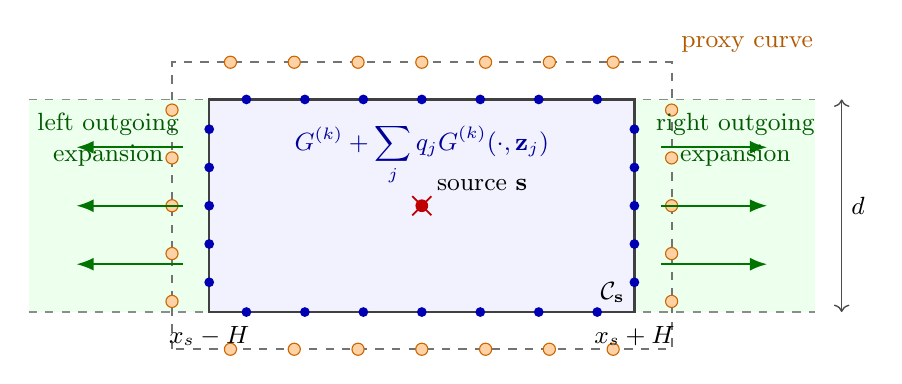
\begin{tikzpicture}[
    x=1.35cm,
    y=1.35cm,
    every node/.style={font=\small},
    cell/.style={draw=black!75, line width=0.8pt, fill=blue!5},
    proxybox/.style={draw=black!55, dashed, line width=0.75pt},
    periodicwall/.style={draw=black!45, dashed, line width=0.6pt},
    colloc/.style={circle, fill=blue!70!black, inner sep=1.25pt},
    proxy/.style={circle, draw=orange!80!black, fill=orange!35, inner sep=1.55pt},
    ray/.style={-{Latex[length=2.2mm]}, draw=green!45!black, line width=0.8pt},
    dim/.style={<->, draw=black!70, line width=0.5pt}
  ]
    \fill[green!7] (-3.7,-1) rectangle (-2,1);
    \fill[green!7] (2,-1) rectangle (3.7,1);
    \draw[periodicwall] (-3.7,-1) -- (3.7,-1);
    \draw[periodicwall] (-3.7,1) -- (3.7,1);
    \draw[cell] (-2,-1) rectangle (2,1);
    \draw[proxybox] (-2.35,-1.35) rectangle (2.35,1.35);

    \foreach \x in {-1.8,-1.2,-0.6,0,0.6,1.2,1.8} {
      \node[proxy] at (\x,-1.35) {};
      \node[proxy] at (\x,1.35) {};
    }
    \foreach \y in {-0.9,-0.45,0,0.45,0.9} {
      \node[proxy] at (-2.35,\y) {};
      \node[proxy] at (2.35,\y) {};
    }

    \foreach \x in {-1.65,-1.1,-0.55,0,0.55,1.1,1.65} {
      \node[colloc] at (\x,-1) {};
      \node[colloc] at (\x,1) {};
    }
    \foreach \y in {-0.72,-0.36,0,0.36,0.72} {
      \node[colloc] at (-2,\y) {};
      \node[colloc] at (2,\y) {};
    }

    \foreach \y in {-0.55,0,0.55} {
      \draw[ray] (-2.25,\y) -- (-3.25,\y);
      \draw[ray] (2.25,\y) -- (3.25,\y);
    }

    \fill[red!75!black] (0,0) circle (2.3pt);
    \draw[red!75!black, line width=0.65pt] (-0.09,-0.09) -- (0.09,0.09);
    \draw[red!75!black, line width=0.65pt] (-0.09,0.09) -- (0.09,-0.09);

    \node[above right=2pt] at (0,0) {source $\mathbf{s}$};
    \node[above left] at (2,-1) {$\mathcal C_{\mathbf{s}}$};
    \node[orange!70!black, above right] at (2.35,1.35) {proxy curve};
    \node[green!35!black, align=center] at (-2.95,0.62)
      {left outgoing\\expansion};
    \node[green!35!black, align=center] at (2.95,0.62)
      {right outgoing\\expansion};
    \node[blue!60!black, align=center] at (0,0.48)
      {$G^{(k)}+\displaystyle\sum_j q_jG^{(k)}(\cdot,\mathbf z_j)$};

    \node[below] at (-2,-1.04) {$x_s-H$};
    \node[below] at (2,-1.04) {$x_s+H$};

    \draw[dim] (3.95,-1) -- (3.95,1);
    \node[right] at (3.95,0) {$d$};
    % \node[align=center] at (0,1.67)
    %   {$u(x,y_s+d/2)=e^{\ii\beta d}u(x,y_s-d/2)$};
  \end{tikzpicture}
  \caption{MFS construction of the $y$-quasiperiodic Green's function. Proxy
  sources represent the smooth correction inside the bounded cell, while
  Rayleigh expansions impose outgoing behavior in the two unbounded
  $x$-directions.}
  \label{fig:y-qpgreen-mfs}
\end{figure}

For truncation order
$M$, the MFS approximation is
\begin{align}
  G_{\mathrm{QP}}^{(k)}(\mathbf{x},\mathbf{s})\approx
  \begin{cases}
    \displaystyle
    \sum_{m=-M}^{M}c_m^+
    e^{+\ii\gamma_m(X-H)}\psi_m(Y),
    & X>H,\ |Y|\leq d/2,\\[0.6em]
    \displaystyle
    G^{(k)}(\mathbf{x},\mathbf{s})
    +\sum_{j=1}^{N_p}q_jG^{(k)}(\mathbf{x},\mathbf{z}_j),
    & |X|\leq H,\ |Y|\leq d/2,\\[0.6em]
    \displaystyle
    \sum_{m=-M}^{M}c_m^-
    e^{-\ii\gamma_m(X+H)}\psi_m(Y),
    & X<-H,\ |Y|\leq d/2.
  \end{cases}
  \label{eq:y-qpgreen-mfs-ansatz}
\end{align}
The $\pm$ sign in the exponent of the Rayleigh expansions is chosen to ensure that the outgoing condition is satisfied, i.e., left-going waves for left half-guide and right-going waves for right half-guide.
The representation is extended from this strip to all $y$ by quasiperiodicity.

% \subsection{Determination of the coefficients}
The unknown proxy strengths $q_j$ and Rayleigh coefficients $c_m^\pm$
are determined by collocation. At paired points on the horizontal boundaries,
the near-field expression $G_{\mathrm{near}}$ in the middle line of
\eqref{eq:y-qpgreen-mfs-ansatz} is required to satisfy
\begin{align}
  G_{\mathrm{near}}(X,d/2)
  &=e^{\ii\beta d}G_{\mathrm{near}}(X,-d/2),\\
  \partial_YG_{\mathrm{near}}(X,d/2)
  &=e^{\ii\beta d}\partial_YG_{\mathrm{near}}(X,-d/2).
\end{align}
On the two artificial vertical boundaries, it is matched in both value and
$x$-derivative to the far-field expression $G_{\mathrm{far}}$ in the top and bottom lines of \eqref{eq:y-qpgreen-mfs-ansatz}:
\begin{align}
  G_{\mathrm{near}}(H,Y)&=G_{\mathrm{far}}(H,Y),&
  \partial_XG_{\mathrm{near}}(H,Y)&=\partial_XG_{\mathrm{far}}(H,Y),\\
  G_{\mathrm{near}}(-H,Y)&=G_{\mathrm{far}}(-H,Y),&
  \partial_XG_{\mathrm{near}}(-H,Y)&=\partial_XG_{\mathrm{far}}(-H,Y).
\end{align}
Collocating these equations produces a linear, generally overdetermined system
for $\{q_j\}$ and $\{c_m^\pm\}$, which is solved in the least-squares sense.
Once these coefficients are known, \eqref{eq:y-qpgreen-mfs-ansatz} gives the
Green's function in the central cell and its outgoing continuation into both
unbounded sides. No volumetric mesh or truncation of the unbounded
$x$-direction is required.

\section{Bloch-mode construction of outgoing trace subspaces}
In this section we construct the outgoing trace spaces used in the center-cell
formulation. The main idea is to first compute the scattering matrix of a
single periodic guide cell, then convert its scattering relation into a
generalized eigenvalue problem for the Bloch multipliers. The decaying Bloch
modes selected from this eigenproblem provide a finite-dimensional basis for
the outgoing Cauchy traces on \(\Gamma^\pm\).

\subsection{Scattering matrix}
As a priliminary to the Bloch mode construction, we introduce the scattering matrix $S^\pm$
of a single cell $\mathcal{C}^\pm$. Generally, we consider an arbitary cell 
$\mathcal{C} = [X_\mathrm{L}, X_\mathrm{R}] \times [0,d]$ with two vertical boundaries $\Gamma_\mathrm{L}$, $\Gamma_\mathrm{R}$ and inclusion $\Omega$ in it.
We have shown that the y-quasiperiodic field in the 
homogeneous background near the two vertical artificial boundaries has the form \eqref{eq:homogeneous-field}, let $a, b \in \mathbb{C}^\mathbb{Z} \times \mathbb{C}^\mathbb{Z}$ 
be the Rayleigh amplitudes on the left and right boundaries, respectively. That is, 
\begin{align*}
  u_\mathrm{L}[a](x,y) = \sum_{m\in\mathbb{Z}} a_m^\rightarrow e^{\ii \gamma_m (x - X_\mathrm{L})} \psi_m(y) + \sum_{m\in\mathbb{Z}} a_m^\leftarrow e^{-\ii \gamma_m (x - X_\mathrm{L})} \psi_m(y),\\
  u_\mathrm{R}[b](x,y) = \sum_{m\in\mathbb{Z}} b_m^\rightarrow e^{\ii \gamma_m (x - X_\mathrm{R})} \psi_m(y) + \sum_{m\in\mathbb{Z}} b_m^\leftarrow e^{-\ii \gamma_m (x - X_\mathrm{R})} \psi_m(y).
\end{align*}
The incident waves are right-going waves on the left boundary and left-going waves on the right boundary, and the outgoing waves are left-going waves on the left boundary and right-going waves on the right boundary. We can define the scattering matrix: 
\begin{align}
  S: \mathbb{C}^\mathbb{Z} \times \mathbb{C}^\mathbb{Z} \to \mathbb{C}^\mathbb{Z} \times \mathbb{C}^\mathbb{Z},\quad
  \begin{bmatrix}
    a^\rightarrow\\
    b^\leftarrow
  \end{bmatrix}
  \mapsto
  \begin{bmatrix}
    a^\leftarrow\\
    b^\rightarrow
  \end{bmatrix},\quad
  S = \begin{bmatrix}
    R_\mathrm{L} & T_{\mathrm{RL}}\\
    T_{\mathrm{LR}} & R_\mathrm{R}
  \end{bmatrix},
\end{align}
or equivalently,
\begin{equation}
  \label{eq:scattering-blocks}
  \begin{aligned}
    a^\leftarrow &= R_\mathrm{L}a^\rightarrow + T_{\mathrm{RL}}b^\leftarrow,\\
    b^\rightarrow &= T_{\mathrm{LR}}a^\rightarrow + R_\mathrm{R}b^\leftarrow.
  \end{aligned}
  \end{equation}
Here \(R_\mathrm{L}\) maps a wave incident from the left boundary to the
reflected wave on the left boundary, while \(T_{\mathrm{LR}}\) maps the same
left-incident wave to the transmitted wave on the right boundary. The blocks
\(R_\mathrm{R}\) and \(T_{\mathrm{RL}}\) are defined analogously for incidence
from the right boundary. For the lead cells \(\mathcal C^\pm\), the same
definitions give the corresponding blocks of \(S^\pm\).

The scattering matrix can be assembled one column at a time. For example, prescribing the \(n\)-th left incident Rayleigh channel means \(a^\rightarrow=e_n\) and \(b^\leftarrow=0\); the computed reflected and transmitted amplitudes form the corresponding column of \(R_\mathrm{L}\) and \(T_{\mathrm{LR}}\). Right incidence is treated analogously.
In numerical implementation, we truncate the Rayleigh basis to \(-M\leq m\leq M\), and set \(K=2M+1\), then $S \in \mathbb{C}^{2K\times 2K}$. Next we show how to determine $M$ and compute the columns of $S$. For demonstrative purposes, we consider the left incidence case. The right incidence case is similar. We take \begin{align*}
  e^{\ii \gamma_n (x - X_\mathrm{L})} \psi_n(y) = \frac{1}{\sqrt{d}} e^{\ii \gamma_n (x - X_\mathrm{L})} e^{\ii \beta_n y}
\end{align*}
as the incident wave, i.e., $a = [e_n; 0]$, then we can solve \begin{align*}
  A_\mathrm{QP}\eta = -B_{\partial \Omega} a
\end{align*}
to obtain the density $\eta$ of the layer potential of the scattered field, then we need 
to convert the layer potential representation to the Rayleigh expansion near the 
two vertical boundaries. We make use of the spectral representation of the y-quasiperiodic Green's function \eqref{eq:qp-green-spectral},
let $\mathbf{s} = (x_s, y_s)$ be some boundary point of $\Omega$. To get the $n$-th column of $R_\mathrm{L}$ and $T_{\mathrm{LR}}$, we rewrite \eqref{eq:qp-green-spectral} as \begin{align*}
  G_\mathrm{QP}^{(k)}(x,y;x_s,y_s) &= \frac{\ii}{2\sqrt{d}} \sum_{m\in\mathbb{Z}} \frac{1}{\gamma_m} e^{-\ii \beta_m y_s + \ii \gamma_m (x_s - X_\mathrm{L})} e^{-\ii \gamma_m (x - X_\mathrm{L})} \psi_m(y),\quad x < x_s,\\
  &= \frac{\ii}{2\sqrt{d}} \sum_{m\in\mathbb{Z}} \frac{1}{\gamma_m} e^{-\ii \beta_m y_s - \ii \gamma_m (x_s - X_\mathrm{R})} e^{\ii \gamma_m (x - X_\mathrm{R})} \psi_m(y),\quad x > x_s.
\end{align*}
And the normal derivative is: \begin{align*}
  &\frac{\partial G_\mathrm{QP}^{(k)}}{\partial \nu(\mathbf{s})}(x,y;x_s,y_s) \\
  ={}& \frac{\ii}{2\sqrt{d}} \sum_{m\in\mathbb{Z}} \frac{1}{\gamma_m} (\ii \gamma_m \nu_x(\mathbf{s}) - \ii \beta_m \nu_y(\mathbf{s})) e^{-\ii \beta_m y_s + \ii \gamma_m (x_s - X_\mathrm{L})} e^{-\ii \gamma_m (x - X_\mathrm{L})} \psi_m(y),\quad x < x_s,\\
  ={}& \frac{-\ii}{2\sqrt{d}} \sum_{m\in\mathbb{Z}} \frac{1}{\gamma_m} (\ii \gamma_m \nu_x(\mathbf{s}) + \ii \beta_m \nu_y(\mathbf{s})) e^{-\ii \beta_m y_s - \ii \gamma_m (x_s - X_\mathrm{R})} e^{\ii \gamma_m (x - X_\mathrm{R})} \psi_m(y) ,\quad x > x_s.
\end{align*}
Now we can compute the Rayleigh amplitudes by replace the kernel in the layer potential with the corresponding coefficients functions of $\mathbf{s}$ in the above two equations.
For example: \begin{multline}
(R_\mathrm{L})_{mn} = \int_{\partial \Omega} \frac{\ii}{2\sqrt{d}\gamma_m} e^{-\ii \beta_m y_s + \ii \gamma_m (x_s - X_\mathrm{L})} \sigma(\mathbf{s})\,\dd s(\mathbf{s}) \\
+ \int_{\partial \Omega} \frac{\ii}{2\sqrt{d}\gamma_m} (\ii \gamma_m \nu_x(\mathbf{s}) - \ii \beta_m \nu_y(\mathbf{s})) e^{-\ii \beta_m y_s + \ii \gamma_m (x_s - X_\mathrm{L})} \tau(\mathbf{s})\,\dd s(\mathbf{s}),
\end{multline}
and similarly:\begin{multline}
(T_{\mathrm{LR}})_{mn} = \int_{\partial \Omega} \frac{\ii}{2\sqrt{d}\gamma_m} e^{-\ii \beta_m y_s - \ii \gamma_m (x_s - X_\mathrm{R})} \sigma(\mathbf{s})\,\dd s(\mathbf{s}) \\
+ \int_{\partial \Omega} \frac{-\ii}{2\sqrt{d}\gamma_m} (\ii \gamma_m \nu_x(\mathbf{s}) + \ii \beta_m \nu_y(\mathbf{s})) e^{-\ii \beta_m y_s - \ii \gamma_m (x_s - X_\mathrm{R})} \tau(\mathbf{s})\,\dd s(\mathbf{s}),
\end{multline}
where the indices $m$ and $n$ run from $-M$ to $M$. The other two blocks of the scattering matrix can be computed analogously.

\subsection{Bloch modes}
From definition~\ref{def:bloch-mode}, we know that a Bloch mode reproduces its total directional state after one outward cell up to a multiplier $\lambda$, using the notation in the previous subsection, we have
\begin{align*}
  \phi_\lambda(X_\mathrm{R}, y) = \lambda \phi_\lambda(X_\mathrm{L},y),
\end{align*}
or \begin{align*}
  b = \lambda a \quad \text{or equivalently}\quad a = \lambda^{-1} b,
\end{align*}
we use the first one, substituting it into \eqref{eq:scattering-blocks}, we obtain
the following generalized eigenvalue problem for the Bloch multiplier $\lambda$ and the corresponding Rayleigh amplitudes $a = a(\lambda)$:
\begin{align}
  \begin{bmatrix}
    -R_\mathrm{L} & I \\ T_\mathrm{LR} & 0
  \end{bmatrix}\begin{bmatrix}
    a^\rightarrow \\ a^\leftarrow
  \end{bmatrix}
   = \lambda \begin{bmatrix}
    0 & T_\mathrm{RL} \\ I & -R_\mathrm{R}
  \end{bmatrix}\begin{bmatrix}
    a^\rightarrow \\ a^\leftarrow
  \end{bmatrix}.
\end{align}
The Bloch mode $\phi_\lambda$ corresponding to the multiplier $\lambda$ has the Rayleigh expansion in the neighborhood of the left boundary $\Gamma_\mathrm{L}$ as follows:
\begin{align*}
  \phi_\lambda(x,y) = \sum_{m\in\mathbb{Z}} a_m^\rightarrow(\lambda) e^{\ii \gamma_m (x - X_\mathrm{L})} \psi_m(y) + \sum_{m\in\mathbb{Z}} a_m^\leftarrow(\lambda) e^{-\ii \gamma_m (x - X_\mathrm{L})} \psi_m(y).
\end{align*}
To determine the admissible Bloch modes, we need to check the Bloch multiplier $\lambda$,
for the right half-guide, $|\lambda| < 1$ is admissible; and for the left half-guide, $|\lambda^{-1}| < 1$ is admissible\footnote{The case of $|\lambda| = 1$ is left for future work.}. 

In numerical implementation, we truncate the Rayleigh basis to \(-M\leq m\leq M\), and set \(K=2M+1\), then the generalized eigenvalue problem has dimension $2K$. Solving the generalized eigenvalue problem gives a set of $(\phi_j, \lambda_j)$, and the truncated
trace $\operatorname{Tr} \phi_j \in \mathbb{C}^{2K}$. The outgoing trace subspace is: 
\begin{align}
  \mathcal{E}^+_\mathrm{out} = \operatorname{span}\{\operatorname{Tr}_{\Gamma^+} \phi_j: |\lambda_j| < 1\},\quad \mathcal{E}^-_\mathrm{out} = \operatorname{span}\{\operatorname{Tr}_{\Gamma^-} \phi_j: |\lambda_j| > 1\} \subset \mathbb{C}^{2K}.
\end{align}
The case of $|\lambda| = 1$ is left for future work. A possible approach is to use the limiting absorption principle, i.e., adding a small imaginary part to the wavenumber $k$ and then taking the limit as the imaginary part goes to zero.

\section{Numerical results}
All of the numerical experiments are implemented in MATLAB R2023a on MacBook Pro with Apple M3 Pro chip and 18GB memory. The codes are available at subfolder \texttt{examples}.

\subsection{Convergence of the MFS construction}
The experiment in this subsection is implemented by the script
\path{examples/run_qpgreen_linton_tables.m}. It compares the MFS construction
of the \(y\)-quasiperiodic Green's function with an Ewald reference at the
three single-point parameter choices reported in Tables 2--4 of
Linton~\cite{Linton1998}. The Linton tables are used only to set the values of
\(kd\), \(\beta d\), the evaluation point \((X/d,Y/d)\), and the Ewald
truncation parameters.

The MFS parameters are fixed for all three cases: period \(d=1\), source point
\(\mathbf{s}=(0,0)\), cell half-width in the non-periodic direction \(H=0.6\),
Rayleigh half-truncation \(M=16\), number of Rayleigh modes \(2M+1=33\), total
number of proxy sources \(N_{\mathrm{proxy}}=160\), distance from the cell box
to the proxy box \(\delta_{\mathrm{proxy}}=0.15\), collocation points on each
periodic boundary \(N_{\mathrm{side}}=160\), and collocation points on each
artificial vertical boundary \(N_{\mathrm{top}}=160\). Thus the least-squares system has
\(N_{\mathrm{proxy}}+2(2M+1)=226\) unknowns and
\(2N_{\mathrm{side}}+4N_{\mathrm{top}}=960\) matching equations. The Ewald
parameters follow Linton's notation: Ewald splitting parameter \(a=2\),
spectral truncation \(M_1\), spatial-image truncation \(M_2\), and
exponential-integral expansion order \(N\). We use Linton's table-specific
choices: \((M_1,M_2,N)=(3,2,7)\) for Table 2, \((4,2,28)\) for Table 3, and
\((3,2,7)\) for Table 4.

\begin{table}[htbp]
  \centering
  \caption{Single-point comparison of the MFS and Ewald quasiperiodic Green
  function values on Linton Tables 2--4. Times are in seconds.}
  \label{tab:linton-mfs-ewald}
  \resizebox{\textwidth}{!}{%
  \begin{tabular}{c c c c c c c c}
    \hline
    Linton table
    & \(kd\)
    & \(\beta d\)
    & \((X/d,Y/d)\)
    & \(|G_{\mathrm{MFS}}-G_{\mathrm{Ewald}}|\)
    & relative error
    & Ewald time
    & MFS time \\
    \hline
    2
    & \(2\)
    & \(\sqrt{2}\)
    & \((0,0.01)\)
    & \(3.8655\times10^{-12}\)
    & \(6.6854\times10^{-12}\)
    & \(2.401\times10^{-3}\)
    & \(7.4877\times10^{-2}\) \\
    3
    & \(10\)
    & \(5\sqrt{2}\)
    & \((0,0.01)\)
    & \(4.7724\times10^{-11}\)
    & \(1.2064\times10^{-10}\)
    & \(6.64\times10^{-4}\)
    & \(4.7915\times10^{-2}\) \\
    4
    & \(2\)
    & \(3\)
    & \((0,0.01)\)
    & \(3.7673\times10^{-12}\)
    & \(4.9456\times10^{-12}\)
    & \(2.951\times10^{-3}\)
    & \(5.1065\times10^{-2}\) \\
    \hline
  \end{tabular}}
\end{table}

Using the Table 2 parameter set, the script
\path{examples/run_qpgreen_table2_grid_error.m} also compares the MFS and
Ewald Green-function values on a uniform grid in one \(y\)-periodic cell. The
grid is
\[
  (x,y)\in[-H,H]\times[-d/2,d/2],
  \qquad
  H=0.6,\quad d=1,
\]
with the source point excluded from the error statistics. 

\begin{figure}[htbp]
  \centering
  \SafeIncludeGraphics[width=0.68\textwidth]{figs/qpgreen_table2_grid_logerr.png}
  \caption{Grid error for the Table 2 \(y\)-quasiperiodic Green-function
  test. The plotted quantity is
  \(\log_{10}|G_{\mathrm{MFS}}-G_{\mathrm{Ewald}}|\), with the source point
  excluded.}
  \label{fig:table2-qpgreen-grid-error}
\end{figure}

The MFS time in Table~\ref{tab:linton-mfs-ewald} includes both the proxy
precomputation and the single target evaluation. The precomputation dominates
the single-point timing: the three runs have precomputation times
\(0.070644\), \(0.047027\), and \(0.050294\) seconds, while the corresponding
evaluation-only times are \(4.233\times10^{-3}\), \(8.88\times10^{-4}\), and
\(7.71\times10^{-4}\) seconds. This is the expected cost profile for the MFS
construction, since the same proxy solve is reused when many source-target
pairs are evaluated in the boundary-integral matrix assembly.

\subsection{1D periodic waveguide}
In this subsection, we consider a special case of line-defected waveguide, in which case
\(\Omega^\pm = \varnothing\), and \(\Omega^0\) is a star-shaped inclusion, as
shown in Figure~\ref{fig:1d-waveguide-inclusion}. The experiment is
implemented by the script \path{examples/run_tep_fixed_beta_k_scan.m}. This is
a standard 1D periodic waveguide model. In this case the Bloch modes are exactly the Rayleigh modes\begin{align*}
  e^{\ii \gamma_m |x|}e^{\ii \beta_m y},\quad m\in\mathbb{Z}.
\end{align*}
Since $\gamma_m$ are chosen such that $\Im \gamma_m \geq 0$, the multiplier $|e^{\ii \gamma_m L}| < 1$ if and only if $\Im \gamma_m > 0$, i.e. $\beta_m^2 > k^2$. Let 
$\mathcal{C}^0 = [-H, H] \times [-d/2, d/2]$, which is symmetric about $x$-axis, thus
we only need to scan $\beta$ in the first irreducible Brillouin zone \([0,\pi/d]\). 
If we search $k$ in the interval $[0, \beta)$, then all of the Rayleigh modes are
outgoing/admissible and the quasiperiodic Green's function decays in the $x$-direction.
In this notation, the region \(k\geq \beta\) is the \emph{light cone}
\cite[Chapter~7]{Joannopoulos2011}. This is the
same distinction used in projected band diagrams: below the light cone the
background admits no propagating radiation channel, while inside the light cone
there are extended states in the exterior medium. Equivalently, for
\(\beta\in[0,\pi/d]\) and \(k<\beta\), every Rayleigh shifted wave number
\(\beta_m=\beta+2\pi m/d\) satisfies \(|\beta_m|>k\). Thus, after the numerical
truncation \(|m|\leq M\), the outgoing trace space is spanned by the decaying
Rayleigh modes in the retained channels. This observation is special to
the homogeneous 1D periodic waveguide; for a general periodic half-guide, the
outgoing modes must be selected from the cell Bloch multipliers rather than
from a single Rayleigh-channel inequality.

\begin{figure}[htbp]
\centering
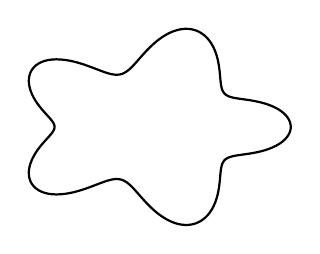
\begin{tikzpicture}[scale=5]
  \draw[thick]
    plot[
      domain=0:360,
      samples=240,
      smooth,
      variable=\t
    ]
    ({0.3*cos(\t) + 0.03*cos(6*\t) + 0.03*cos(4*\t)},
     {0.2*sin(\t) + 0.03*sin(6*\t) - 0.03*sin(4*\t)});
\end{tikzpicture}
\caption{Star-shaped inclusion used for \texttt{flag\_geom = 'star'} in the
numerical experiment. Its parametrization is given by:
\[
  x(t)=0.3\cos t+0.03\cos 6t+0.03\cos 4t,\qquad
  y(t)=0.2\sin t+0.03\sin 6t-0.03\sin 4t,
  \quad 0\leq t<2\pi .
\]}
\label{fig:1d-waveguide-inclusion}
\end{figure}

For a fixed Bloch phase \(\beta\), we scan the wavenumber \(k\) by evaluating
\(\sigma_{\min}(\Aqp(k,\beta))\). The algorithm first samples a coarse global
grid on the prescribed \(k\)-interval and detects strict local dips. Each
retained dip is then refined recursively: on each refinement level, an odd
local grid is placed on the current bracket, the grid point with the smallest
singular value is selected, and the next bracket is chosen as the interval
between its two neighboring grid points. If the minimum occurs at an endpoint,
the bracket is expanded subject to the original \(k\)-bounds. This procedure is
applied first at a mid resolution and then at the final boundary resolution.

The MFS parameters are the same as in the previous subsection:
\[
  H=0.6,\qquad \delta_{\mathrm{proxy}}=0.15,\qquad
  N_{\mathrm{side}}=N_{\mathrm{top}}=160,\qquad
  N_{\mathrm{proxy}}=160,\qquad M=16 .
\]
The remaining important parameters are
\[
  d=1,\qquad \beta=\pi,\qquad n_{\mathrm{ref}}=\sqrt{13},\qquad
  k\in[0.01\beta,0.99\beta],
\]
with boundary discretizations
\[
  N_{\partial\Omega}^{\mathrm{coarse}}=40,\qquad
  N_{\partial\Omega}^{\mathrm{mid}}=60,\qquad
  N_{\partial\Omega}^{\mathrm{final}}=100.
\]
The global scan uses \(400\) grid points. Each recursive refinement uses
\(11\) local grid points, with minimum and maximum refinement levels \(6\) and
\(8\), respectively. Local dips no larger than \(100\) times the best coarse
dip are retained, at most \(20\) candidates are refined, and final candidates
closer than \(10^{-11}\) in \(k\) are merged.

Table~\ref{tab:fixed-beta-timing} reports the cost of one sample evaluation.
The ``proxy'' time is the time for constructing the proxy-source
representation of the quasiperiodic Green function used by the MFS. The
``assembly'' time is the time for forming the matrix \(\Aqp(k,\beta)\) from the
boundary quadrature, layer-potential blocks, and MFS Green-function data. The
``SVD'' time is the time for computing the singular values of the assembled
matrix and extracting \(\sigma_{\min}(\Aqp(k,\beta))\).

\begin{table}[htbp]
  \centering
  \caption{Timing of one \(\sigma_{\min}(\Aqp(k,\beta))\) evaluation at
  \(k=2.1301282065163130\) and \(\beta=\pi\), measured by
  \texttt{examples/run\_tep\_fixed\_beta\_timing.m}. Times are in seconds and
  exclude geometry construction, which is cached in the scan.}
  \label{tab:fixed-beta-timing}
  \begin{tabular}{c c c c c c c}
    \hline
    \(N_{\partial\Omega}\) & matrix size & proxy & assembly & SVD & total
    & \(\sigma_{\min}\) \\
    \hline
    40 & 80 & \(0.05434\) & \(0.06248\) & \(5.655\times10^{-4}\)
    & \(0.1140\) & \(2.611\times10^{-7}\) \\
    60 & 120 & \(0.05114\) & \(0.1036\) & \(1.527\times10^{-3}\)
    & \(0.1560\) & \(8.313\times10^{-10}\) \\
    80 & 160 & \(0.05282\) & \(0.1906\) & \(4.734\times10^{-3}\)
    & \(0.2503\) & \(1.244\times10^{-11}\) \\
    100 & 200 & \(0.04996\) & \(0.2569\) & \(0.01122\)
    & \(0.3162\) & \(1.276\times10^{-13}\) \\
    \hline
  \end{tabular}
\end{table}

\begin{table}[htbp]
  \centering
  \caption{Refined fixed-\(\beta\) candidates from
  \texttt{examples/run\_tep\_fixed\_beta\_k\_scan.m}.}
  \label{tab:fixed-beta-k-scan}
  \begin{tabular}{c c c c c}
    \hline
    rank
    & \(k_\ast\)
    & \(\sigma_{\min}(\Aqp(k_\ast,\beta))\)
    & final width
    & stopping reason \\
    \hline
    1
    & \(2.8480494264121057\)
    & \(1.2531\times10^{-13}\)
    & \(2.5282\times10^{-12}\)
    & relative improvement \\
    2
    & \(2.1301282065163130\)
    & \(1.2763\times10^{-13}\)
    & \(1.0081\times10^{-13}\)
    & max levels \\
    3
    & \(1.4293696359612806\)
    & \(4.4445\times10^{-13}\)
    & \(1.0103\times10^{-13}\)
    & max levels \\
    \hline
  \end{tabular}
\end{table}

\begin{figure}[htbp]
  \centering
  \SafeIncludeGraphics[width=0.68\textwidth]{figs/tep_fixed_beta_k_scan.png}
  \caption{Fixed-\(\beta\) global \(k\)-scan for the 1D periodic waveguide.
  The blue curve shows the coarse scan of
  \(\sigma_{\min}(\Aqp(k,\beta))\), and the red markers show the refined
  candidates listed in Table~\ref{tab:fixed-beta-k-scan}.}
  \label{fig:fixed-beta-k-scan}
\end{figure}

The experiment finds three sharp dips of
\(\sigma_{\min}(\Aqp(k,\beta))\) in the scanned interval. As shown in
Figure~\ref{fig:fixed-beta-k-scan}, the global scan locates the relevant
valleys and the local refinement then resolves the final candidates. The
corresponding values in Table~\ref{tab:fixed-beta-k-scan} reach
\(10^{-13}\)-level singular values at
\(k_\ast\approx 2.8480494264\), \(2.1301282065\), and \(1.4293696360\). The
timing data in Table~\ref{tab:fixed-beta-timing} show that, for the final
resolution \(N_{\partial\Omega}=100\), one evaluation takes about \(0.316\)
seconds, with the dominant cost coming from assembling \(\Aqp(k,\beta)\), while
the dense SVD of the \(200\times 200\) matrix is still comparatively small.

Finally, the same recursive scanning strategy is applied over the
\((\beta,k)\)-plane by the script
\texttt{run\_tep\_band\_structure.m}. The
result is shown in Figure~\ref{fig:tep-band-structure}. The run uses
\(\beta\in[0,\pi]\) with \(80\) Bloch-phase samples and, for each fixed
\(\beta\), enforces \(10^{-6}\leq k\leq \beta-10^{-6}\). Table~\ref{tab:band-scan-counts}
summarizes the number of evaluated \((k,\beta)\) pairs at each boundary
discretization. The total wall-clock time was \(3569.738\) seconds, or
\(59.496\) minutes.

\begin{table}[!htbp]
  \centering
  \caption{Number of evaluated \((k,\beta)\) pairs in the band-structure scan
  from \texttt{run\_tep\_band\_structure.m}. Counts are before
  duplicate sample merging.}
  \label{tab:band-scan-counts}
  \begin{tabular}{c c c}
    \hline
    \(N_{\partial\Omega}\) & role & evaluated \((k,\beta)\) pairs \\
    \hline
    40 & coarse global scan & 10002 \\
    60 & first local refinement & 8613 \\
    100 & final local refinement & 8910 \\
    \hline
    total & all evaluations & 27525 \\
    \hline
  \end{tabular}
\end{table}

\begin{figure}[!htbp]
  \centering
  \SafeIncludeGraphics[width=0.68\textwidth]{figs/tep_band_structure.png}
  \caption{Band-structure scan for the star-shaped one-dimensional periodic
  waveguide. The color shows the clipped value of
  \(\log_{10}\sigma_{\min}(\Aqp(k,\beta))\); darker valleys indicate candidate
  transmission-eigenvalue bands.}
  \label{fig:tep-band-structure}
\end{figure}

After duplicate sample merging, the band-structure data contain \(23004\)
distinct plotted points and \(107\) final refined candidates. The smallest
sampled singular value in this run is approximately \(2.50\times10^{-15}\).

\subsection{Line-Defect waveguide}

\section{Conclusion}

\appendix
\numberwithin{equation}{section}
\titleformat{\section}
  {\normalfont\large\bfseries}
  {\appendixname~\thesection.}{0.5em}{}

\section{Proof of Theorem~\ref{thm:single-cell-representation}}
\label{sec:appendixA}
In this appendix, the superscripts ($+$) and ($-$) no longer label the right
and left half-guides, respectively. Instead, they denote the exterior and
interior traces on \(\partial\Omega\), respectively. Let \(\nu\) be the unit
normal on \(\partial\Omega\) pointing out of \(\Omega\). We define
\begin{align*}
  u^\pm(\mathbf{x})
  &:= \lim_{h \to 0^+}u\bigl(\mathbf{x}\pm h\nu(\mathbf{x})\bigr),\\
  u_\nu^\pm(\mathbf{x})
  &:= \lim_{h \to 0^+}
  \nabla u\bigl(\mathbf{x}\pm h\nu(\mathbf{x})\bigr)\cdot\nu(\mathbf{x}),
  \qquad \mathbf{x}\in\partial\Omega.
\end{align*}

We first recall the free-space Green representation formulas used below; see
\cite[Section~3.2]{ColtonKress1983}. Let
\(\kappa>0\), and suppose that \(u\) is a sufficiently smooth solution of
\[
  (\Delta+\kappa^2)u=0 \qquad \text{in }\Omega.
\]
Then its interior Cauchy data satisfy
\begin{align}
  -\mathcal{S}^{(\kappa)}[u_\nu^-](\mathbf{x})
  +\mathcal{D}^{(\kappa)}[u^-](\mathbf{x})
  =
  \begin{cases}
    -u(\mathbf{x}), & \mathbf{x}\in\Omega,\\
    0, & \mathbf{x}\in\mathbb{R}^2\setminus\overline{\Omega}.
  \end{cases}
  \label{eq:green-representation-interior}
\end{align}
The second line is the corresponding extinction formula: the layer potential
generated by the interior Cauchy data vanishes on the other side of the
interface.

For the exterior formula, suppose instead that \(u\) solves
\[
  (\Delta+\kappa^2)u=0
  \qquad \text{in }\mathbb{R}^2\setminus\overline{\Omega}
\]
and satisfies the two-dimensional Sommerfeld radiation condition
\begin{align}
  \frac{\partial u}{\partial r}-\ii\kappa u
  =o\bigl(r^{-1/2}\bigr),
  \qquad r=|\mathbf{x}|\to\infty,
  \label{eq:sommerfeld-radiation-appendix}
\end{align}
uniformly with respect to the direction \(\mathbf{x}/|\mathbf{x}|\). Its
exterior Cauchy data then give
\begin{align}
  -\mathcal{S}^{(\kappa)}[u_\nu^+](\mathbf{x})
  +\mathcal{D}^{(\kappa)}[u^+](\mathbf{x})
  =
  \begin{cases}
    0, & \mathbf{x}\in\Omega,\\
    u(\mathbf{x}), & \mathbf{x}\in\mathbb{R}^2\setminus\overline{\Omega}.
  \end{cases}
  \label{eq:green-representation-exterior}
\end{align}
Thus the same combination \(-\mathcal{S}^{(\kappa)}u_\nu+
\mathcal{D}^{(\kappa)}u\) reproduces the Helmholtz field on the side from
which the Cauchy data are taken and vanishes on the opposite side, with the
sign determined by whether the data are interior or exterior traces.

We will need the following quasiperiodic analogues.

\begin{lemma}
\label{lem:qp-interior-green-representation}
Let $u$ satisfy $(\Delta+\kappa^2)u=0$ in $\Omega$, then for $(\kappa, \beta)$ not a Wood anomaly, we have\begin{align}
  -\mathcal{S}^{(\kappa)}_\mathrm{QP}[u_\nu^-](\mathbf{x})
  +\mathcal{D}^{(\kappa)}_\mathrm{QP}[u^-](\mathbf{x})
  =
  \begin{cases}
    -u(\mathbf{x}), & \mathbf{x}\in\Omega,\\
    0, & \mathbf{x}\in \mathcal{C}\setminus\overline{\Omega}.
  \end{cases}
\end{align}
\end{lemma}

\begin{proof}
Following the lattice-image argument of
\cite[Appendix~A, Lemma~9]{BarnettGreengard2010}, let
\(\mathbf e_y=(0,1)\), and for each \(j\in\mathbb Z\) define the translated
inclusion and field
\[
  \Omega_j:=\Omega+jd\mathbf e_y,
  \qquad
  u_j(\mathbf z):=u(\mathbf z-jd\mathbf e_y),
  \quad \mathbf z\in\Omega_j.
\]
Then \((\Delta+\kappa^2)u_j=0\) in \(\Omega_j\). By translation invariance of
the free-space Green's function, the lattice-sum definition of the
quasiperiodic potentials gives
\begin{align*}
  &-\mathcal S_\mathrm{QP}^{(\kappa)}[u_\nu^-](\mathbf x)
  +\mathcal D_\mathrm{QP}^{(\kappa)}[u^-](\mathbf x)\\
  &\qquad=
  \lim_{N\to\infty}\sum_{j=-N}^{N}e^{\ii j\beta d}
  \left(
    -\mathcal S_{\partial\Omega_j}^{(\kappa)}[(u_j)_\nu^-](\mathbf x)
    +\mathcal D_{\partial\Omega_j}^{(\kappa)}[u_j^-](\mathbf x)
  \right),
\end{align*}
where the boundary written as a subscript indicates the curve over which the
free-space potential is integrated.

Since the inclusion lies strictly inside the cell, every
\(\mathbf x\in\mathcal C\) lies outside \(\overline{\Omega_j}\) when
\(j\neq0\). The extinction part of
\eqref{eq:green-representation-interior}, applied to \(u_j\) in \(\Omega_j\),
therefore shows that every \(j\neq0\) term in the lattice sum is zero. For
\(j=0\), the same formula gives \(-u(\mathbf x)\) when
\(\mathbf x\in\Omega\) and zero when
\(\mathbf x\in\mathcal C\setminus\overline\Omega\). Thus the only
contribution surviving the lattice-sum limit is the \(j=0\) image, which
proves the stated formula.
\end{proof}


\begin{lemma}
\label{lem:qp-exterior-green-representation}
Let $u$ satisfy $(\Delta+\kappa^2)u=0$ in $\mathcal{C}\setminus\overline{\Omega}$ and the quasiperiodic condition \begin{align*}
  \left. u \right|_{y = d} = e^{\ii \beta d} \left. u \right|_{y = 0}, \quad
\left. \partial_y u \right|_{y = d} = e^{\ii \beta d} \left. \partial_y u \right|_{y = 0}.
\end{align*}
Assume that $(\kappa, \beta)$ is not a Wood anomaly and that \(u\) satisfies the Rayleigh radiation condition, then
\begin{align}
  -\mathcal{S}^{(\kappa)}_\mathrm{QP}[u_\nu^+](\mathbf{x})
  +\mathcal{D}^{(\kappa)}_\mathrm{QP}[u^+](\mathbf{x})
  =
  \begin{cases}
    0, & \mathbf{x}\in\Omega,\\
    u(\mathbf{x}), & \mathbf{x}\in \mathcal{C}\setminus\overline{\Omega}.
  \end{cases} \label{eq:qp-exterior-green-representation}
\end{align}
\end{lemma}

\begin{proof}
We follow the standard method of proof \cite[Theorem~3.3]{ColtonKress1983}. Apply Green's 2nd identity to the domain $\mathcal{C} \setminus \overline{\Omega}$ if 
$\mathbf{x} \in \Omega$, or the domain $\{\mathbf{y} \in \mathcal{C}\setminus \overline{\Omega} : |\mathbf{x} - \mathbf{y}| > \varepsilon\}$ if $\mathbf{x} \in \mathcal{C} \setminus \overline{\Omega}$. In the latter case the limit $\varepsilon \to 0$ is taken, 
and \eqref{eq:lattice-sum-qpgreen} shows that only $j = 0$ term contributes to the limit
of the integral over the circle of radius $\varepsilon$ centered at $\mathbf{x}$. The 
integral over the boundary $\partial \Omega$ gives the layer potential combination.
We will focus on the following integral:\begin{align}
  I = \int_{\partial \mathcal{C}} \frac{\partial G^{(\kappa)}_\mathrm{QP}(\mathbf{x},\mathbf{y})}{\partial \nu(\mathbf{y})} u(\mathbf{y}) - G^{(\kappa)}_\mathrm{QP}(\mathbf{x},\mathbf{y}) u_\nu(\mathbf{y}) \, \dd s(\mathbf{y}).
\end{align}
The integrals over the top and bottom sides of the cell cancel because $G^{(\kappa)}_\mathrm{QP}(\mathbf{x}, \cdot)$ is anti-quasiperiodic, i.e. quasiperiodic with phase 
$e^{-\ii \beta d}$. Suppose $\mathbf{y} = (s,t)$, then we have \begin{align*}
  I_\mathrm{top} &= \int_{X_\mathrm{L}}^{X_\mathrm{R}} \left[e^{\ii \beta d} u(s,0) e^{-\ii \beta d}\partial_t G^{(\kappa)}_\mathrm{QP}(\mathbf{x},(s,0)) - e^{-\ii \beta d} G^{(\kappa)}_\mathrm{QP}(\mathbf{x},(s,0)) e^{\ii \beta d} \partial_t u(s,0) \right] \, \dd s,\\
  I_\mathrm{bottom} &= -\int_{X_\mathrm{L}}^{X_\mathrm{R}} \left[u(s,0) \partial_t G^{(\kappa)}_\mathrm{QP}(\mathbf{x},(s,0)) - G^{(\kappa)}_\mathrm{QP}(\mathbf{x},(s,0))\partial_t u(s,0)\right] \, \dd s,
\end{align*}
which cancel each other. 

The integrals over the left and right sides need to be evaluated carefully. By\eqref{eq:right-coefficient-extraction}--\eqref{eq:right-outgoing-rayleigh-condition},
the Rayleigh radiation condition eliminates the
right-going Rayleigh component at the left boundary, and the left-going Rayleigh component at the right boundary, which implies that $u$ has the form 
\begin{align*}
  u(s,t) &= \sum_{m\in\mathbb Z} a_m^\mathrm{R} e^{\ii\gamma_m (s - X_\mathrm{R})}\psi_m(t), \quad s \geq X_\mathrm{R},\\
  u(s,t) &= \sum_{m\in\mathbb Z} b_m^\mathrm{L} e^{-\ii\gamma_m (s - X_\mathrm{L})}\psi_m(t), \quad s \leq X_\mathrm{L},
\end{align*}
where $a, b$ are given by \eqref{eq:right-coefficient-extraction}--\eqref{eq:left-coefficient-extraction}. Define the anti-quasiperiodic dual modes 
\begin{align*}
  \widetilde{\psi}_m(t) = \frac{1}{\sqrt{d}} e^{-\ii \beta_m t},\quad \int_0^d \psi_m(t) \widetilde{\psi}_n(t) \, \dd t = \delta_{mn}.
\end{align*}
The spectral Green's function formula \eqref{eq:qp-green-spectral}, now viewed as a 
function of $\mathbf{y} = (s,t)$, gives: \begin{align*}
  G^{(\kappa)}_\mathrm{QP}(\mathbf{x},(s,t)) &= \sum_{m\in\mathbb Z} 
  c_m^\mathrm{L}(\mathbf{x}) e^{-\ii \gamma_m (s - X_\mathrm{L})} \widetilde\psi_m(t), \quad s < x_1,\\
  G^{(\kappa)}_\mathrm{QP}(\mathbf{x},(s,t)) &= \sum_{m\in\mathbb Z} 
  c_m^\mathrm{R}(\mathbf{x}) e^{\ii \gamma_m (s - X_\mathrm{R})} \widetilde\psi_m(t), \quad s > x_1,
\end{align*}
where, explicitly, \begin{align*}
  c_m^\mathrm{L}(\mathbf{x}) = \frac{\ii}{2\sqrt{d}\gamma_m} e^{\ii \beta_m x_2} 
  e^{\ii \gamma_m (x_1 - X_\mathrm{L})},\quad 
  c_m^\mathrm{R}(\mathbf{x}) = \frac{\ii}{2\sqrt{d}\gamma_m} e^{\ii \beta_m x_2}
  e^{\ii \gamma_m (X_\mathrm{R} - x_1)}.
\end{align*}
On the right side $s = X_\mathrm{R}$, we have \begin{align*}
  I_\mathrm{right} &= \int_0^d u(X_\mathrm{R},t) \partial_s G^{(\kappa)}_\mathrm{QP}(\mathbf{x},(X_\mathrm{R},t)) - G^{(\kappa)}_\mathrm{QP}(\mathbf{x},(X_\mathrm{R},t))\partial_s u(X_\mathrm{R},t)  \, \dd t\\
  &= \sum_{m,n} a_m^\mathrm{R} c_n^\mathrm{R}(\mathbf{x}) \ii(\gamma_n - \gamma_m) \int_0^d \psi_m(t) \widetilde{\psi}_n(t) \, \dd t = 0.
\end{align*}
An identical calculation gives $I_\mathrm{left} = 0$. Thus the integral over the boundary of the cell vanishes, the representation formula \eqref{eq:qp-exterior-green-representation} holds, and the proof is complete.
\end{proof}

Now we are ready to prove Theorem~\ref{thm:single-cell-representation}.
\begin{proof}[Proof of Theorem~\ref{thm:single-cell-representation}]
We prove the existence and uniqueness seperately.

\emph{1. Existence.}
In a homogeneous neighborhood of $\Gamma_\mathrm{L}$ not intersecting $\overline{\Omega}$,
field $u$ has unique Rayleigh expansion \begin{align*}
  u(x, y) = \sum_{m \in \mathbb{Z}} \left[ a_m^\mathrm{L}e^{\ii\gamma_m (x - X_\mathrm{L})} + b_m^\mathrm{L}e^{-\ii\gamma_m (x - X_\mathrm{L})} \right] \psi_m(y), 
\end{align*}
the Rayleigh coefficients $a_m^\mathrm{L}$ and $b_m^\mathrm{L}$ are given by \eqref{eq:right-coefficient-extraction}--\eqref{eq:left-coefficient-extraction} since $(k, \beta)$ is not a Wood anomaly.
In the neighborhood of $\Gamma_\mathrm{R}$ we can extract the Rayleigh coefficients $a_m^\mathrm{R}$ and $b_m^\mathrm{R}$ in a similar way. We define the homogeneous 
background component $u_h$ as following:
\begin{align}
  u_h(x, y) = \sum_{m \in \mathbb{Z}} \left[ a_m^\mathrm{L}e^{\ii\gamma_m (x - X_\mathrm{L})} + b_m^\mathrm{R}e^{-\ii\gamma_m (x - X_\mathrm{R})} \right] \psi_m(y),
\end{align}
and define \begin{align}
  w = \begin{cases}
    u - u_h, & \mathbf{x} \in \mathcal{C}\setminus\overline{\Omega},\\
    u, & \mathbf{x} \in \Omega,
  \end{cases}
\end{align}
satisfying the Rayleigh radiation condition \eqref{eq:left-outgoing-rayleigh-condition}--\eqref{eq:right-outgoing-rayleigh-condition}. 


We introduce the (swapped-wavenumber) transmission problem: \begin{align}
  \begin{cases}
  (\Delta + k^2) v = 0& \quad \text{in } \Omega,\\
  (\Delta + n^2k^2) v = 0& \quad \text{in } \mathbb{R}^2 \setminus \overline{\Omega},\\
  \frac{\partial v}{\partial r} - \ii n k v = o(r^{-1/2}),& \quad r = |\mathbf{x}| \to \infty,\\
  v^+ - v^- = f,&\\
  v_\nu^+ - v_\nu^- = g,&
  \end{cases}
  \label{eq:swapped-transmission-problem}
\end{align}
where $f$ and $g$ are given continuous functions on $\partial \Omega$, in our construction 
we take
\begin{align*}
  f = -w^+ - w^-; \qquad g = -w_\nu^+ - w_\nu^-,
\end{align*}
then the transmission problem has a unique solution $v$ by \cite[Theorem~3.41]{ColtonKress1983}.
Define the densities\begin{align*}
  \tau = w^+ - v^- = -w^- - v^+;\qquad \sigma = -w^+_\nu + v_\nu^- = w^-_\nu + v_\nu^+,
\end{align*}
It remains to verify that these densities produce the prescribed fields $w$. 
For $\mathbf{x} \in \Omega$, the Green's representation formulae \eqref{eq:green-representation-interior} and \eqref{eq:green-representation-exterior} give
\begin{align*}
  &\mathcal{S}^{(nk)}[\sigma](\mathbf{x}) + \mathcal{D}^{(nk)}[\tau](\mathbf{x})\\
  ={}& -\left[ -\mathcal{S}^{(nk)}[w_\nu^-](\mathbf{x}) + \mathcal{D}^{(nk)}[w^-](\mathbf{x}) \right] - \left[ -\mathcal{S}^{(nk)}[v_\nu^+](\mathbf{x}) + \mathcal{D}^{(nk)}[v^+](\mathbf{x}) \right]\\
  ={}& -[-w(\mathbf{x})] - 0 = w(\mathbf{x}), \qquad \mathbf{x} \in \Omega.
\end{align*}
For $\mathbf{x} \in \mathcal{C} \setminus \overline{\Omega}$, Lemma~\ref{lem:qp-interior-green-representation} and Lemma~\ref{lem:qp-exterior-green-representation} give
\begin{align*}
  &\mathcal{S}^{(k)}_\mathrm{QP}[\sigma](\mathbf{x}) + \mathcal{D}^{(k)}_\mathrm{QP}[\tau](\mathbf{x})\\
  ={}& \left[ -\mathcal{S}^{(k)}_\mathrm{QP}[w_\nu^+](\mathbf{x}) + \mathcal{D}^{(k)}_\mathrm{QP}[w^+](\mathbf{x}) \right] - \left[ -\mathcal{S}^{(k)}_\mathrm{QP}[v_\nu^-](\mathbf{x}) + \mathcal{D}^{(nk)}_\mathrm{QP}[v^-](\mathbf{x}) \right]\\
  ={}& w(\mathbf{x}) - 0 = w(\mathbf{x}), \qquad \mathbf{x} \in \mathcal{C} \setminus \overline{\Omega}.
\end{align*}
This proves existence.

\emph{2. Uniqueness.}
Suppose that
\[
  u=u_h+w=\widehat u_h+\widehat w
  \qquad\text{in }\mathcal C\setminus\overline\Omega
\]
are two decompositions of the stated form. Then
\[
  \widehat u_h-u_h=w-\widehat w.
\]
The right-hand side is outgoing at both ports. The left-hand side is a
homogeneous background field of the form \eqref{eq:homogeneous-field}, whose
only incoming coefficients are
$\widehat\xi_m^\rightarrow-\xi_m^\rightarrow$ at the left port and
$\widehat\xi_m^\leftarrow-\xi_m^\leftarrow$ at the right port. Since it is
also outgoing, all these coefficients vanish. Hence
$\widehat u_h=u_h$ and $\widehat w=w$. The interface densities are then
unique by the same complementary-field uniqueness argument used in their
construction above.

To prove the uniqueness of the densities $\sigma, \tau$, suppose that $w = 0$ in 
$\mathcal{C} \setminus \partial \Omega$, and define the complementary field over 
the whole plane minus $\partial \Omega$
\begin{align}
  v(\mathbf{x}) = \begin{cases}
    \mathcal{S}^{(k)}_\mathrm{QP}[\sigma](\mathbf{x}) + \mathcal{D}^{(k)}_\mathrm{QP}[\tau](\mathbf{x}), & \mathbf{x} \in \Omega,\\
    -\mathcal{S}^{(nk)}[\sigma](\mathbf{x}) - \mathcal{D}^{(nk)}[\tau](\mathbf{x}), & \mathbf{x} \in \mathbb{R}^2 \setminus \overline{\Omega}.
  \end{cases}
\end{align}
Then $w^- = w^-_\nu = 0$ and by the jump relations of 
$\mathcal{S}^{(nk)}[\sigma]+ \mathcal{D}^{(nk)}[\tau]$ we have $v^+ = -\tau$ and $v_\nu^+ = \sigma$. Similarly, since $w^+ = w^+_\nu = 0$ by the jump relations of $\mathcal{S}^{(k)}_\mathrm{QP}[\sigma]+ \mathcal{D}^{(k)}_\mathrm{QP}[\tau]$ we have $v^- = -\tau$ and $v_\nu^- = \sigma$.
It's easy to check that $v$ solves the transmission problem 
\eqref{eq:swapped-transmission-problem} with $f = g = 0$. By the uniqueness of the transmission problem, we have $v \equiv 0$ in $\mathbb{R}^2 \setminus \partial \Omega$, 
from which the jump relations back to the $w$ imply $\sigma = \tau = 0$. This proves the uniqueness of the densities.
\end{proof}


\bibliographystyle{plain}
\bibliography{references}
\end{document}
